\chapter{Algorithms for Implementing MMQL}
\label{algorithms}

Having proposed a multi-model query language called MMQL in~\cref{mmql}, in theory we could now start writing queries encompassing multiple data models.
However, designing such a language is only half the work.
Naturally, for a query language to be useful, it must also be executable.
Designing the supporting algorithms which are necessary for the implementation of a query language is far from trivial, which is why we will spend a considerable amount of effort describing them in this chapter.
A very rough basis of an approach for unified multi-model querying based on category theory was first outlined by Pavel Koupil and Irena Holubov{\'a}~\cite{unified_representation} as part of the potential future applications of their proposed unified categorical representation of multi-model data.
This chapter builds on their initial ideas, developing them into a set of fully-fledged algorithms which support the implementation of our proposed query language -- MMQL.

As the implementation effort itself is also non-trivial, we will separate it into a separate chapter altogether, and in this chapter, we will only focus on the design of the algorithms themselves.
The algorithms presented in this chapter form the basis of \textit{MM-quecat}, a proof-of-concept implementation of MMQL described in~\cref{quecat}.

\section{Proposed approach}
\label{algorithms:section:approach}

Since we want to reuse existing database systems as they are, our querying approach must necessarily rely on the translation of MMQL queries into queries in the databases' native query languages, subsequently transforming the retrieved data into our categorical representation.
However, to enable us to reason better about the whole approach, let us first describe it from a very high level view.
As such, we can divide our proposed approach into the following steps:

\begin{enumerate}
    \item \textit{Create a set of query plans.} Analyze the query and prepare a plan of which data from which databases should be used during the query execution. In the case of data redundancy, multiple alternative query plans are created.
    \item \textit{Create a join plan for each query plan.} Given a query plan, joining data from different databases may be required. The point of a join plan is to define the join points for the query plan, as well as the data which will be necessary from both ends of the join point to perform the actual join.
    \item \textit{Select the best query plan.} If there are multiple possible query plans due to data redundancy, the best query plan must be selected by the query planner, if a specific plan was not explicitly requested by the user. Note that this step may need to come after the query part translation step instead if the query planner needs to use the generated native queries to make an estimation of the cost of the entire query.
    \item \textit{Process individual query parts.} If we consider a query part to be a self-contained unit of execution, we need to translate it into a database-native query. We define query parts in such a way that it is always possible to translate a single query part into a single native query.
    \item \textit{Merge query part results.} When we have the native database query for each query part, we need to execute it, transform the result into the categorical representation, and merge the retrieved data together.
    \item \textit{Perform projection on the result.} After merging all query part results into a single one (corresponding to the contents of the entire \texttt{WHERE} clause of the query), we need to project the results to the desired final representation as described by the \texttt{SELECT} clause, before returning them to the user. Also, there may be some MMQL statements which cross database boundaries, which makes them impossible to execute fully within the context of a single query part. Therefore we need to execute these deferred statements in this step.
    \item \textit{Transform the result into the desired format.} Since an instance category may not be the desired output format for many use cases, this optional step lets users specify which format the query results should be returned in, like JSON or RDF.
\end{enumerate}

An example of a query being processed may be seen in~\cref{fig:queryworkflow}. The steps as shown in the diagram do not correspond one-to-one to the steps outlined in this chapter, but the overall flow is the same.
\cref{fig:queryworkflow} comes from a conference demo paper which the author of this thesis coauthored  with Pavel Koupil and Irena Holubov{\'a}, but which is not yet published at the time of writing of this thesis~\cite{mm_quecat}.

As we will see later on in this chapter, a number of tradeoffs were involved in the formation of this version of the proposed approach.
Since MMQL and its supporting algorithms are attempting to break new ground in a sparsely studied area, our main goals for this approach were \textit{simplicity} and \textit{comprehensibility}, with performance not being a large focus point.
Considering we are proposing one of the first ever unified querying solutions for the multi-model, multi-database environment, we are aware that any solution we propose at this stage will have limitations and weaknesses, which is why we focus on designing a simple solution first, analyzing its limitations, and pointing out what may be improved by future works on this topic.

\begin{figure}
\centering
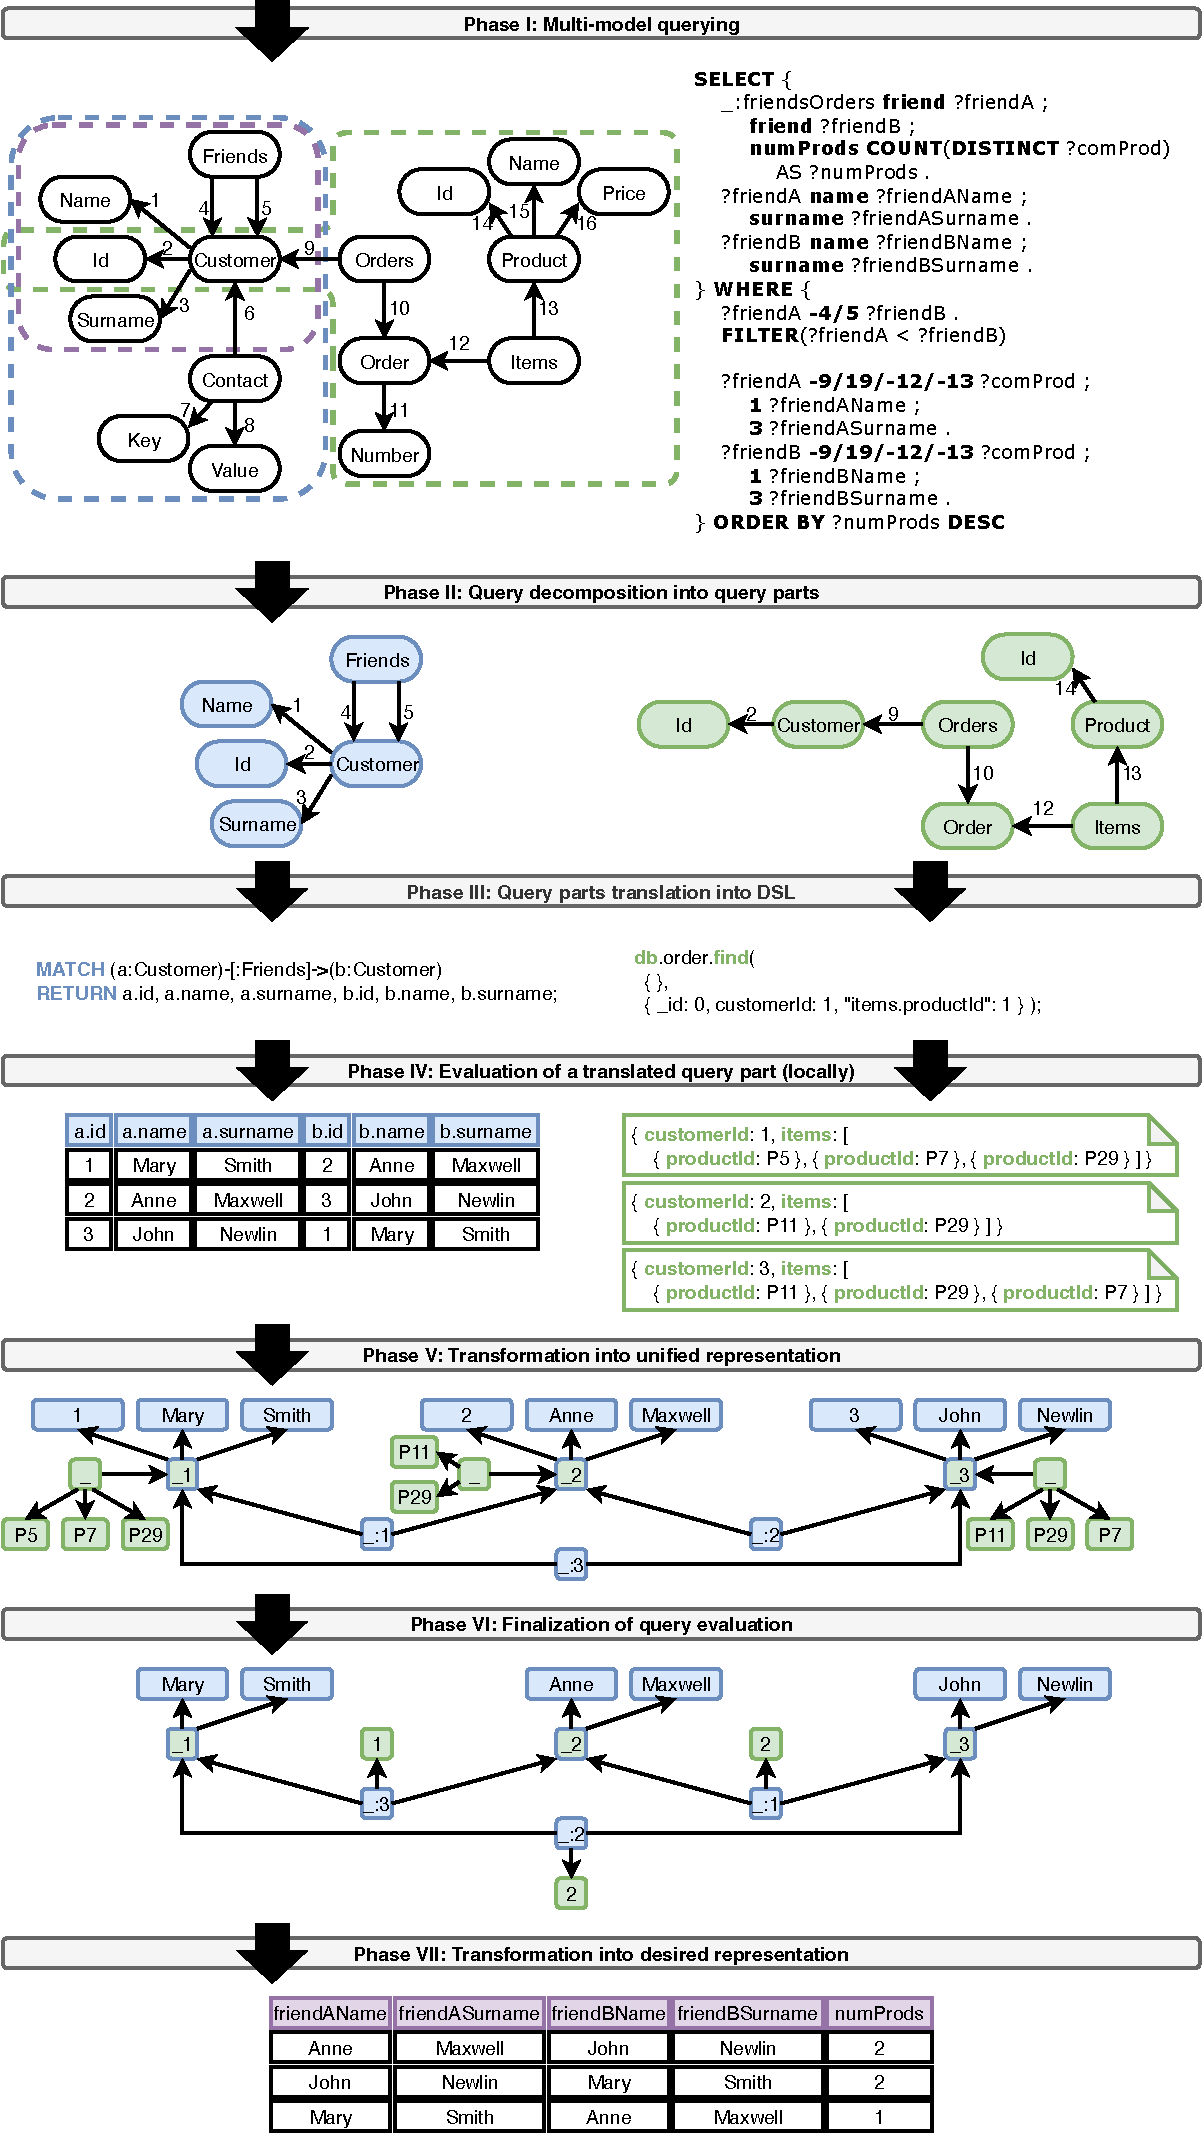
\includegraphics[width=0.9\textwidth]{img/query-workflow.pdf} 
\caption{A diagram showing the full querying workflow~\cite{mm_quecat}.}
\label{fig:queryworkflow}
\end{figure}

\subsection{Database Wrappers}
\label{algorithms:subsection:wrappers}

As we divide the MMQL query into separate query parts, the idea is for each query part to be a self-contained unit of execution which compiles down to a single native database query, regardless of the specific database.
We also wish to design our algorithms to be \textit{database agnostic}, as the spectrum of multi-model databases is vast, and we do not want to confine ourselves to a specific set of them.
Both of these facts motivate the concept of \textit{database wrappers}, which encapsulate the specifics of each database and its native query language behind a generic interface.
As the general idea of the wrappers is encapsulation of database-specific logic, we have two main requirements for the design of this generic interface:

\begin{itemize}
    \item The interface should be general enough to allow the addition of any database system which we may reasonably expect to support;
    \item The interface should abstract away all categorical concepts from the wrappers' implementations where possible to make supporting new databases easier; and
    \item The order in which wrapper interface methods are called should be irrelevant.
\end{itemize}

Perhaps the last goal is worth elaborating on -- since MMQL allows the definition of statements in any order, it is also desirable for our query translation algorithm to be able to process these statements in any order.
For this reason, all methods in the wrapper interface will make the wrapper simply "remember" this operation, and finally, when the entire query is processed, a finalization method will be called on the wrapper, building the native query.
In this way, the database wrappers operate similarly to a builder object in the builder design pattern~\cite{gof}.
With these goals in mind, we propose the following methods for the generic database wrapper interface:

\begin{itemize}
    \item \texttt{defineKind($kindId$, $kindName$)} which is an initialization function, assigning the identifier $kindId$ to the kind name $kindName$. The kind name refers to for example table names in PostgreSQL or collection names in MongoDB. Note that a single kind name can be registered multiple times under different identifiers, in which case its data is retrieved independently multiple times.
    \item \texttt{addProjection($propertyPath$, $kindId$, $variableId$)} which adds projection of a specific property to a query, i.e. given a specific kind, this method will add the specified property of this kind to the native query output.
    \item \texttt{addFilter($variableId$, $filterOp$, $constant$)} which constrains the value of a property identified by $variableId$ to a logical relation specified by $filterOp$ (such as equality or inequality), using $constant$ as the second operand. Note that the variable $variableId$ does not need to exist before this method is called, as the validation is delayed until the moment of generation of the native query. In addition, we also consider an overload \texttt{addFilter($propertyPath$, $kindId$, $filterOp$, $constant$)} which does not require its filtered property to be a part of the projection, instead specifying the path directly. This overload is necessary because of triples which contain constant literals.
    \item \texttt{addFilter($variableId_1$, $filterOp$, $variableId_2$)} which creates a relationship between the values of two variables, eliminating solutions where this relationship is not satisfied. This can be used together with aggregations, whose results have their own variable identifiers.
    \item \texttt{addValueSet($variableId$, $constants$)} which constrains the value of a property identified by $variableId$ to the set of values provided in $constants$.
    \item \texttt{addJoin($kindId_1$, $kindId_2$, $joinProperties$)} which performs a join operation on the two kinds provided. Note that we call it a join operation, but for example, in the case of the graph model, this entails a graph traversal rather than a join in the relational sense.
    \item \texttt{addRecursiveJoin($recursiveJoinPath$)} which performs a series of recursive joins between various kinds in the query part (if recursion is supported). If we have a morphism with repetition, its domain must necessarily be the same as its codomain, otherwise it would not be possible to repeat it. This kind of recursive joining is useful in cases of transitive relationship traversal (for example finding all superiors of a given company employee), and it is generally supported in the relational model with recursive common table expressions\footnote{\url{https://www.postgresql.org/docs/current/queries-with.html}}, and in the graph model with variable length paths\footnote{\url{https://neo4j.com/docs/cypher-manual/current/syntax/patterns/\#cypher-pattern-varlength}}.
    \item \texttt{addAggregation($aggregationType$, $aggregationRootKindId$,\\$rootIdPaths$, $kindId$, $propertyPath$, $variableId$)} which performs an aggregation of the specified type on the specified property of the specified kind. The aggregation may have multiple possible roots (for example averaging the item price for a set of customers, each of whom has made multiple orders with multiple items - should we average the items per order, or per customer?), and for this reason, the aggregation root is also specified, along with one of its identifiers. The result of this aggregation is stored in the variable identified by $variableId$.
    \item \texttt{buildQuery()} which takes the information collected from all method calls on this wrapper and generates the native database query based on it. This method contains the majority of the actual wrapper logic, with the other methods mostly just storing the arguments for processing by this method. The result of this method is a tuple ($nativeQuery$, $variableMap$), where $nativeQuery$ is the built native query in a string representation, and $variableMap$ contains a map of variable identifiers included in the projection to property paths within the native query result.
\end{itemize}

Naturally, not all databases support all of these operations, for example Cassandra does not support joins\footnote{We only consider the built-in capabilities of the given databases, not user-defined procedures.}.
For this reason, each database wrapper also exposes the following properties about the functionality the underlying database has:

\begin{itemize}
    \item \texttt{isJoinSupported} which specifies whether the database supports (inner) joins. For example, most relational databases do, as do graph databases in the form of graph traversals. Document databases may support joins, but for example MongoDB only supports left outer joins. Naturally, the inner join operation can be emulated using the left join operation, but the wrapper implementer may not want to support this due to the involved complexity. Finally, some databases like Cassandra do not support joins of any kind.
    \item \texttt{isOptionalJoinSupported} which specifies whether the database supports optional (left outer) joins. This is necessary because of the \texttt{OPTIONAL} clause in MMQL. In the situation that optional joins are not supported, the joins must be performed at the categorical level.
    \item \texttt{isNonIdFilterSupported} which specifies whether the database supports filtering of properties outside of the identifier set of the root object of a given kind. For example, many key-value databases treat stored values as opaque objects, not allowing filtering based on their value, but only their retrieval.
    \item \texttt{isCountAggregationSupported} which specifies whether the database supports the \texttt{COUNT} aggregation. We also define a corresponding property for each type of aggregation supported in MMQL.
    \item \texttt{isRecursionSupported} which specifies whether the database supports recursive queries, which may necessitate the recursive joining of kinds. Such joins are generally supported in relational and graph databases, and allow the traversal of tree or graph structures in a single query.
\end{itemize}

For each interface method mentioned, we will also define an optional counterpart which means that this operation should be included in the query, but with optional semantics.
In some cases, the implementations will be identical (for example in SQL, adding projection on an optional column will return \texttt{NULL} if that column is not set for a particular row).
However, in some cases, there may be differences (for example in SQL, we would generate an inner join for a non-optional join operation, whereas we would generate a left outer join in the optional case).
When defining the interface methods, we used a set of arguments which must also be explained in detail:

\begin{itemize}
    \item $propertyPath$ is an ordered list of property names, forming a traversal from the kind root to a leaf property. This property path, along with name information (for example, whether the name is dynamic), also carries the property type at each level, in order to allow database wrappers to correctly deal with nested objects and arrays. The argument $rootIdPaths$ is a list of property paths.
    \item $kindId$ is the identifier of the kind to which this operation applies. This identifier can be mapped to the kind name configured in the database wrapper at initialization time. The inclusion of an identifier instead of a name allows us to query the same kind multiple times within a query part, for example joining customers together with other customers based on the equality of their names. Similarly, $kindName$ refers to the name of the kind identified by $kindId$ in its respective database.
    \item $variableId$ identifies the output field of the native query. We cannot generally make assumptions about how the query output may be structured, as this decision is ultimately up to the database wrapper. For this reason, whenever defining a property which should be part of the native query output, we assign it a variable identifier. When the native query is compiled, the database wrapper returns a mapping of variable identifiers to concrete property paths within the query output, allowing us to parse this output into a categorical representation correctly.
    \item $joinProperties$ contains a set of tuples, with each tuple containing a property path within the corresponding kind. These tuples define join points for the join operation. Note that a limitation of our approach is that we only support joins on \textit{equality}. In theory though, joins with more complicated conditions could also be supported. 
    \item $aggregationType$ specifies the type of aggregation which should be performed, like counting or averaging.
    \item $recursiveJoinPath$ is a list of join path segments, where each join path segment may either be a tuple ($kindId_1$, $kindId_2$, $joinProperties$) symbolizing a join between two kinds, a path segment with a repetition specifier ($?$, $*$ or $+$ as in regular expressions), or multiple path segments chained together. In this way, we can represent arbitrary morphism paths with repetitions as sequences of joins between kinds, with some subsequences optionally repeated as necessary. Note that whenever a path segment is repeated, its first kind must be the same as its last kind in order for the repetition to be valid.
\end{itemize}

With the database wrapper interface specified, we can see that in its simplest form, implementing a database wrapper is actually rather straightforward.
In order to support a new database in the most minimal form possible, we can simply implement the function \texttt{addProjection}, at which point we will be able to query any data from this database, even though we would not be able to filter this data or perform joins and aggregations at the database level, forcing them to be executed in a slower way at the instance category level.

\section{Algorithms}

In~\cref{algorithms:section:approach}, we described the high-level steps involved in our proposed approach for the implementation of MMQL.
In this section, we will examine the outlined steps in greater detail, specifying a concrete algorithm for each, as well as discussing the presented algorithms and their weaknesses.

Before we start discussing the particulars of the individual algorithms, we need to discuss one key characteristic of our proposed approach.
As we attempted to divide the whole approach into a number of well-defined, easily digestible algorithms, we were faced with a decision.
On one hand, we could try to propose an algorithm which attempts to translate the query as a whole into native database queries, taking into account all parts of the MMQL query such as projection and ordering.
However, as we discovered during the design process, such an approach would result in a monolithic, very complex algorithm which is hard to reason about, making its modifications or analysis impractical.
For this reason, we opted for a simplification in this matter -- when creating a query plan and dividing the query into query parts, we only consider the contents of the query's \texttt{WHERE} clause, as this clause is actually the only truly necessary part for the retrieval of data from databases.
In this way, we are able to limit the query part translation algorithm to a set of graph patterns and a few other concepts.
This has some implications for the possible performance of our approach, as all query elements outside the scope of the \texttt{WHERE} clause must be handled by the MMQL query engine, which is undoubtedly much less efficient than using native database queries where possible.
However, as a whole, this allowed us to greatly simplify and modularize the proposed algorithms.

In general, we will discuss performance optimization possibilities when presenting the algorithms, but we will not include these optimizations in the algorithms themselves for the sake of simplicity.

\subsection{Query Preprocessing}
\label{algorithms:subsection:preprocessing}

As mentioned in the introduction to this chapter, when constructing native database queries, we will only consider the \texttt{WHERE} clause of the MMQL query.
However, before we proceed with the main parts of the querying process, we need to perform a couple of additional steps first.
One thing which needs to be done is general adjustments to the query structure to make its processing easier in the following steps.
However, as the \texttt{WHERE} clause has the semantics of inducing a schema category, we will also need to construct this schema category for further usage.
In addition to constructing this schema category, we will also need to construct the corresponding mappings.
Lastly, query validation should be a part of this process, like the validation of variable types.
We will not present any validation algorithms as they would be relatively straightforward, and for the rest of this chapter, we will assume that input queries are well formed and valid.
The full query preprocessing algorithm is shown in~\cref{algo:alg:preprocessing}, and we will shortly discuss its constituent parts in greater detail.

\subsubsection{Query Modifications}

In~\cref{mmql} during the introduction of MMQL, we mentioned its power in the form of graph patterns, including constructs like ending triples with a semicolon instead of a period to repeat the same subject in multiple triples.
However, as these constructs are simply syntactic sugar, we convert them to sets of triples with an explicitly specified subject to simplify their further processing (lines 1-9 in \cref{algo:alg:preprocessing}).

\begin{algorithm}
\small
\DontPrintSemicolon
\SetKwProg{Fn}{function}{:}{}
\SetKw{return}{return}

\KwIn{$\mathbf{SELECT}$  -- query SELECT clause\;} 
\myinput{$\mathbf{WHERE}$ -- query WHERE clause\;}

\ForEach{\textup{graph pattern $P$ in $SELECT \cup WHERE$}}{
    \If{\textup{$P$ has repeated subject $subject$ and morphism $morphism$}}{
        delete $P$ from query

        \ForEach{\textup{$object$ in $P$}}{
            add triple $subject$ $morphism$ $object$ to query
        }
    }
    \ElseIf{\textup{$P$ has repeated subject $subject$}}{
        delete $P$ from query
        
        \ForEach{\textup{$morphism$, $object$ in $P$}}{
            add triple $subject$ $morphism$ $object$ to query
        }
    }
}

\ForEach{\textup{triple $subject$, $morphism$, $object$ in $WHERE$}}{
    \If{\textup{$morphism$ is compound and not repeated}}{
        $b$ := getBaseMorphisms($morphism$)
        
        delete triple $subject$ $morphism$ $object$ from $WHERE$

        $prevVar$ := $subject$
        
        \ForEach{\textup{$baseMorphism$ in $b$}}{
            \If{\textup{$baseMorphism$ is the last element in $b$}}{
                $newVar$ := $object$
            }
            \Else{
                $newVar$ := getUniqueVarName()
            }
            
            add triple $prevVar$ $baseMorphism$ $newVar$ to $WHERE$
        }
    }
}

\ForEach{\textup{triple $subject$, $morphism$, $object$ in $WHERE$}}{
    \If{\textup{$morphism$ is base}}{
        \If{\textup{$morphism$ is $- oppositeMorphism$}}{
            delete triple $subject$ $morphism$ $object$

            add triple $object$ $oppositeMorphism$ $subject$
        }
    }
}

\caption{Query Preprocessing Algorithm.}
\label{algo:alg:preprocessing}
\end{algorithm}

The most interesting part of the query preprocessing step is \textit{compound morphism decomposition} (lines 10-20 in \cref{algo:alg:preprocessing}).
Recall that in MMQL, we may specify compound morphisms using the syntax \texttt{55/31}, meaning the traversal of morphism with signature \texttt{55}, followed by the traversal of morphism with signature \texttt{31}.
Again, as we attempt to make the query processing simple, we decompose all compound morphisms into base morphisms\footnote{For the purposes of the algorithms in this chapter, we will consider base morphisms to be traversals of a base morphism in any direction.}, inserting technical temporary variables with unique names in between the base morphisms.
An example of this can be seen in~\cref{algo:figure:decomposition}, where we can see a triple containing a compound morphism, and the decomposed representation of this triple.
As far as MMQL is concerned, both of these constructs are semantically equivalent.
Finally, for each morphism, we can also traverse it in the opposite direction with the MMQL unary minus operator.
Without loss of generality, we can reverse the direction of traversal for base morphisms along with swapping the subject and object, which simplifies further processing of these opposite-direction traversals (lines 21-25 in \cref{algo:alg:preprocessing}).

\begin{figure}[ht]
\begin{code}
WHERE {
    // Compound morphism before preprocessing
    ?customer 55/31 ?orderNumber .

    // Decomposed compound morphism with inserted variable
    ?customer 55 ?51d747110d95 .
    ?51d747110d95 31 ?orderNumber .
}
\end{code}
\caption{Compound morphism decomposition.}\label{algo:figure:decomposition}
\end{figure}

Note that compound morphism decomposition only applies to compound morphisms without repetition.
When morphisms with repetition are encountered, they are left intact, as it may be necessary to form recursive queries in this instance, and it is not possible to decompose morphisms with infinite upper bound repetition.

The inquisitive reader may raise the question of optimization -- is it possible for the query engine to omit "useless" data along the path of the compound morphism, only retrieving the data necessary for the query variables?
However, recall~\cref{categorical:chapter} where we introduced the notion of the schema and instance category.
The instance category must conform to its corresponding schema category, meaning that if our schema category has base morphisms \texttt{55} and \texttt{31}, these morphisms must also exist as instance morphisms, making this kind of optimization impossible if we intend to stick with the categorical model throughout the process.
Not all hope is lost though, as there is a way to make this optimization work.
If the query engine notices that a particular set of morphisms is only ever traversed together in a compound morphism, it could perform a contraction of these morphisms in the schema category, defining a new schema category where this compound morphism is transformed into a single base morphism.
In this fashion, the instance category would now contain the formerly compound morphism as a base morphism, allowing the query engine to omit irrelevant data from the query plan.

\subsubsection{Constructing the Schema Category}

As we mentioned in the introduction of this subsection, before we may continue with the rest of the process, we must first construct the schema category induced by the \texttt{WHERE} clause, which will be used in the following subsections.
The original schema category which the query was made with is therefore only used as the input for the algorithm for the construction of the schema category induced by the \texttt{WHERE} clause, which we will introduce shortly.
The same applies to the original mappings, which must also be adjusted.
However, before we explain \textit{how} this is done, we should mention \textit{why} it needs to be done.
In fact, if we have a query which contains a maximum of one variable per schema object, this step is totally unnecessary.
The reason for the existence of this step is queries which have multiple variables corresponding to the same schema object (for example, recall~\cref{mmql:figure:samevar}, showing a query selecting two different customers who purchased an item with the same name).
In this case, we need a way to separate the values of both variables, as their possible sets of values may not be the same.

To solve the issue of multiple variables per schema object, we propose a modification to the original schema category.
We will not provide an explicit algorithm for this, as its creation from the following definitions is straightforward.
Let $\mathbf{S}$ = $(\mathcal{O}_\mathbf{S}, \mathcal{M}_\mathbf{S}, \circ_\mathbf{S})$ be the original schema category (recall~\cref{categorical:section:schema}), and let $\mathbf{Var}_{WHERE}$ be the set of variables in the query \texttt{WHERE} clause.
We will define $\mathbf{S}_{WHERE}$ := $(\mathcal{O}_{\mathbf{S}_W}, \mathcal{M}_{\mathbf{S}_W}, \circ_{\mathbf{S}_W})$
For each $var \in \mathbf{Var}_{WHERE}$ and $o \in \mathcal{O}_\mathbf{S}$, we define a schema object $o_{var} \in \mathcal{O}_{\mathbf{S}_W}$ whose instances will contain the values of variable $var$.
Additionally, as the query does not need to contain all (or any) identifiers of any particular schema object which is part of the query, we also add all schema objects necessary for all identifiers of all objects $o_{var} \in \mathcal{O}_{\mathbf{S}_W}$ to $\mathcal{O}_{\mathbf{S}_W}$.
These additional objects are inserted separately for each $o_{var} \in \mathcal{O}_{\mathbf{S}_W}$, they are not shared in the case that multiple variables refer to the same schema object in $\mathbf{S}$.

For each $o_{var1}, o'_{var2} \in \mathcal{O}_{\mathbf{S}_W}$ and $m = (s, o, o', min, max) \in \mathcal{M}_\mathbf{S}$, if the triple \texttt{?var1 s ?var2} exists in the \texttt{WHERE} clause, then we define\\ $m_{var12} := (s_{var12}, o_{var12}, o'_{var12}, min, max) \in \mathcal{M}_{\mathbf{S}_W}$.
In addition, just as we did with schema objects, we will define the required morphisms to satisfy all identifiers of all $o_{var} \in \mathcal{O}_{\mathbf{S}_W}$ to be part of $\mathcal{M}_{\mathbf{S}_W}$.
Using these definitions, we will also consider morphism signatures $s$ to be equivalent to $s_{var12}$ when used in triples of the form \texttt{?var1 s ?var2} in the rest of this chapter when working with $\mathbf{S}_{WHERE}$.
This allows us to reason more simply about the query processing algorithms, as we can keep using signatures specified in the query to refer to corresponding signatures from $\mathbf{S}_{WHERE}$, since given a triple, this mapping is always unambiguous.

Finally, we define $\circ_{\mathbf{S}_W}$ to be the natural extension of $\circ_\mathbf{S}$ over $\mathcal{M}_{\mathbf{S}_W}$.
We show an example of the construction of this induced schema category using a schema category shown in \cref{algo:fig:induced_cat_original} and a query shown in \cref{algo:fig:induced_query}, with the schema category induced by the query's \texttt{WHERE} clause being shown in \cref{algo:fig:induced_cat_new}.
Note that the \texttt{Surname} schema object is missing, as it is not part of the query's \texttt{WHERE} clause, nor is it part of any object's $ids$.

\begin{figure}
\centering
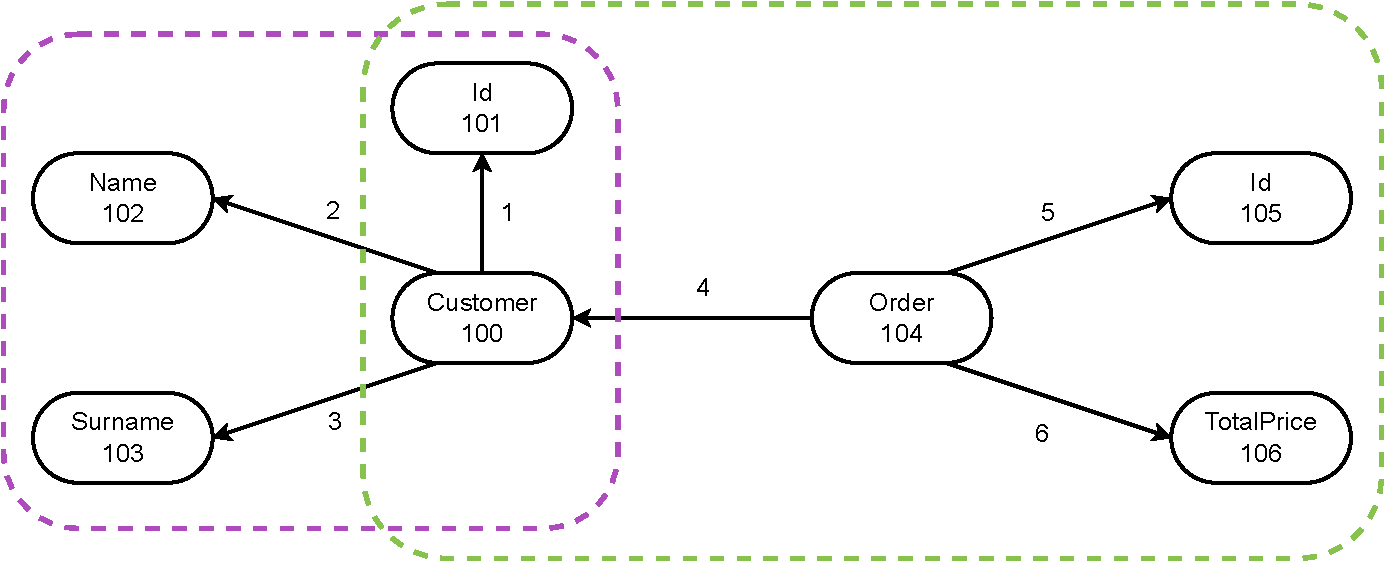
\includegraphics[width=\textwidth]{img/induced-category-original.pdf} 
\caption{A sample schema category showing a set of customers in a relational database, and a set of orders in a document database, with each order containing the identifier of the ordering customer.}
\label{algo:fig:induced_cat_original}
\end{figure}

\begin{figure}
\begin{code}
SELECT {
    _:shared name ?sharedName ;
        price ?sharedPrice .
}
WHERE {
    ?customer1 2 ?sharedName ;
        -4 ?order1 .

    ?customer2 2 ?sharedName ;
        -4 ?order2.

    ?order1 6 ?sharedPrice .
    ?order2 6 ?sharedPrice .
}
\end{code}
\caption{A query returning two customers with the same name who placed an order with the same total price, corresponding to the schema category shown in \cref{algo:fig:induced_cat_original}.}\label{algo:fig:induced_query}
\end{figure}

\begin{figure}
\centering
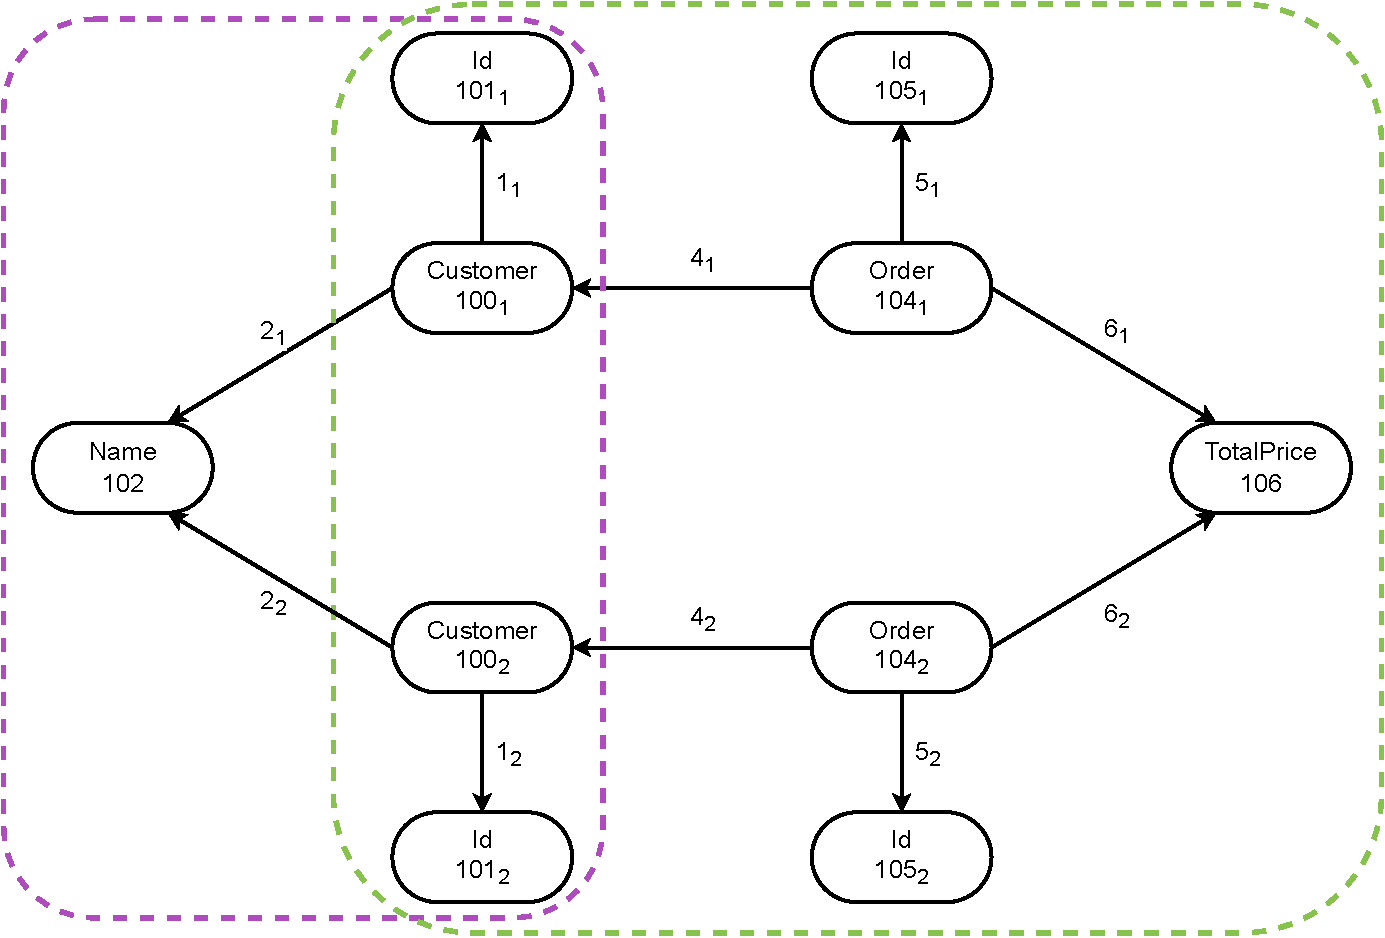
\includegraphics[width=\textwidth]{img/induced-category-new.pdf} 
\caption{Schema category induced by the WHERE clause of the query shown in \cref{algo:fig:induced_query}.}
\label{algo:fig:induced_cat_new}
\end{figure}

We need to mention that the \texttt{WHERE} clause may contain the \texttt{OPTIONAL}, \texttt{UNION} and \texttt{MINUS} clauses in addition to graph patterns and filters.
As far as the generation of the new schema category goes, \texttt{OPTIONAL} is quite simple, as we simply consider its contents the same way as non-optional graph patterns, save for modifying the morphism cardinality at join points to have a minimum of zero, as the optional parts may or may not exist.
It is remarkably similar for \texttt{MINUS}, where we can treat the forbidden pattern as an optional pattern, using it to filter the final result set.
In the case of \texttt{UNION}, we simply consider both of its operands to be optional as far as the schema category is concerned.

As for nested queries, they are evaluated recursively from the most nested to the least nested, and their results are joined to the containing query's \texttt{WHERE} clause.
This means that at the level of the schema category, we simply need to define the appropriate schema objects corresponding to the results of the nested query.

\subsubsection{Constructing New Mappings}

With the new schema category $\mathbf{S}_{WHERE}$ in hand, we naturally also need to adjust the set of mappings $\mathfrak{M}$ corresponding to $\mathbf{S}$ to be valid for $\mathbf{S}_{WHERE}$.
This is necessary because these modified mappings $\mathfrak{M}_{WHERE}$ will be used for the generation of query plans and the translation of query parts to native database queries, both of which operate on the $\mathbf{S}_{WHERE}$ schema category.
Before continuing, it is recommended that the reader is intimately familiar with the concepts introduced in~\cref{categorical:section:mapping}.
It is also worth remembering that for queries with at most one variable per schema object, this operation is effectively a no-op, and its purpose is to correctly handle queries with multiple variables per one schema object.

As we mentioned earlier, we restrict our approach to queries for which every property selection from a kind must necessarily contain the entire property path from the root.
For this reason, it is sufficient to examine only kinds whose root objects are present in the query.

Given $\mathfrak{M}$, let us define $\mathfrak{M}_{WHERE}$ in the following way.
For each mapping $\mathfrak{m} \in \mathfrak{M}$ with root object $o$, discard it if its root object is not part of the query.
Otherwise, for each $o_{var} \in \mathcal{O}_{\mathbf{S}_W}$, we define $\mathfrak{m}_{var} \in \mathfrak{M}_{WHERE}$.
For each property $\phi \in \mathfrak{m}$, we define the corresponding property $\phi' \in \mathfrak{m}_{var}$ recursively by replacing occurrences of signatures $s \in \mathbf{S}$ with signatures $s_{varxy} \in \mathbf{S}_{WHERE}$ for the corresponding objects $o_{varx}, o_{vary} \in \mathbf{S}_{WHERE}$.
This formulation seems complicated, but when explained with plain words, it is actually rather straightforward -- for each schema object in $\mathbf{S}_{WHERE}$ which is the root of some kind's mapping, we are simply constructing an equivalent mapping, but using the new variable-specific objects and morphisms from $\mathbf{S}_{WHERE}$.
For example, let us consider a query selecting two different customers, with the customer kind having its own mapping.
This definition would create two instances of this mapping, each for one of the customer variables, in such a way that when querying the customers' data from the database, the correct data ends up in the correct customers' instance objects, taking into account that some may be shared due to the shape of the query.
We can see an example of such mappings in \cref{algo:fig:induced_cat_mappings}, which correspond to the schema category shown in \cref{algo:fig:induced_cat_new}.

\begin{figure}[ht]
\centering
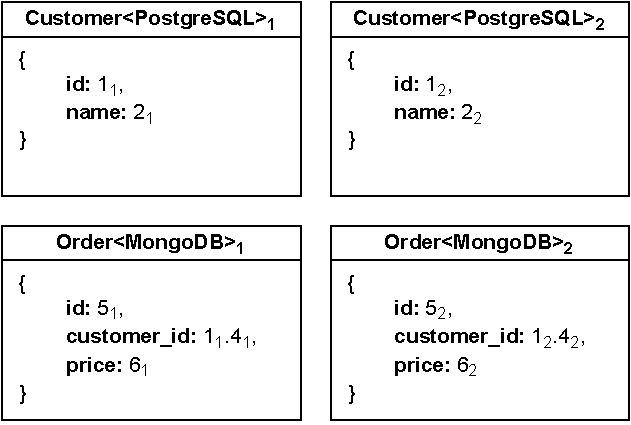
\includegraphics[width=0.75\textwidth]{img/induced-category-mappings.pdf} 
\caption{Mappings corresponding to the induced schema category shown in \cref{algo:fig:induced_cat_new}.}
\label{algo:fig:induced_cat_mappings}
\end{figure}

Note that it may be necessary for a single property $\phi$ to produce multiple properties $\phi'$, $\phi''$ and so on.
This can happen in the specific cases of nested arrays in the mapping, as we are able to bind multiple distinct variables to different elements of the array.
We do not need to give this scenario any special consideration, as long as we presume that given $\phi'$ or $\phi''$, we are able to determine $\phi$, allowing us to correctly construct the appropriate database query during the translation of query parts.

\subsection{Query Plan}
\label{algo:subsection:queryplan}

Now that the query has been preprocessed, the query engine must first create a set of query plans dictating how the query will be executed (recall Phase II in \cref{fig:queryworkflow}).
In simple terms, we consider a query plan to be a plan of which data will be retrieved from which database, and in what way.
When we consider the situation of no data redundancy, we only need to consider a single query plan on the level of MMQL, as there is only one database from which we can retrieve any given kind.
Naturally, the databases' query planners will come into play under the covers, and during the execution of native database queries, the database planners will certainly consider a number of different plans.
However, in the context of MMQL, the query planner only needs to decide where to retrieve the data from, and the optimization of native queries is left up to the databases themselves.
When we consider data redundancy, there will be multiple query plans generated on the MMQL side.

More formally, we consider a query plan to be a set of query parts, such that each distinct base morphism which is part of the MMQL query \texttt{WHERE} clause, is assigned to exactly one query part.
A query part is a set of mappings, assigning base morphisms to kinds defined in mappings.
This means that for each morphism in the query, we make a decision on which kind this morphism should be retrieved from.
The algorithm for the creation of query plans is shown in~\cref{algo:alg:queryplan}.
In simple terms, for each base morphism in the query, it retrieves the set of kinds of which this morphism is a part (lines 1-7), and then generates a set of query plans by Cartesian product of all morphism-kind assignments (lines 8-12).

\begin{algorithm}
\small
\DontPrintSemicolon
\SetKwProg{Fn}{function}{:}{}
\SetKw{return}{return}

\KwIn{$\mathbf{WHERE}$  -- query WHERE clause\;} 
\myinput{$\mathfrak{M}_{WHERE}$  -- set of mappings adjusted for the schema category induced by the WHERE clause\;}

\tcp{Map listing the set of possible source kinds for each morphism}
$morphismKindMap$ := \{\}

$queryPlans$ := [ ]

\ForEach{\textup{triple $subject$ $morphism$ $object$}}{
    \ForEach{\textup{mapping $\mathfrak{m}$ in $\mathfrak{M}_{WHERE}$}}{
        $namePath$ := getPropertyPath($morphism$, $\mathfrak{m}$)

        \If{\textup{$namePath$ is not NULL}}{
            $morphismKindMap$.append($morphism$, $\mathfrak{m}$)
        }
    }
}

$kindAssignments$ := cartesianProduct($morphismKindMap$)

\ForEach{\textup{$kindAssignment$ in $kindAssignments$}}{
    $queryPlan$ := createQueryPlan($kindAssignments$)

    \If{\textup{$queryPlan$ is not NULL}}{
        $queryPlans$.append($queryPlan$)
    }
}


\caption{Query Plan Generation Algorithm.}
\label{algo:alg:queryplan}
\end{algorithm}

There are a couple interesting functions being called in this algorithm which are worth mentioning.
The first of them is \texttt{getPropertyPath}, which given a morphism and a kind's mapping, returns an ordered list of properties which form a traversal from the kind root to the morphism within the kind.
If the morphism does not exist in the kind, this function returns \texttt{NULL}, which is why we can see this function being used to check whether a morphism lies in a given kind.

The next interesting function is \texttt{createQueryPlan}, which may be seen in \cref{algo:alg:createqueryplan}.
This function accepts a mapping of morphisms to their source kinds, and returns a query plan for this mapping.
This function's job is to divide the query into query parts, forming the query plan.
It also validates the query plan, as it only makes sense to assign a morphism to be selected from a kind when the entire property path to this morphism is also being selected from the same kind.
This has a very important consequence for the set of queries which our approach is able to process, as given this constraint, any MMQL query which is only operating on a subforest of a kind's access path which does not include the kind root object is not valid.
For example, given the schema category and access path shown in~\cref{fig:mappings}, a query only selecting order items and their names, but not containing any variable for the \texttt{Order} schema object, would produce zero valid query plans as proposed.
This is fixable by adding special cases for such queries to the algorithm, which might insert the necessary variables for a valid query plan to be generated.
However, we omitted these special cases for the sake of simplicity.

\begin{algorithm}
\small
\DontPrintSemicolon
\SetKwProg{Fn}{function}{:}{}
\SetKw{return}{return}
\SetKw{continue}{continue}

\Fn{\textup{createQueryPlan($kindAssignments$)}}{
\KwIn{$kindAssignments$ -- the source kind for each morphism\;}
    \ForEach{\textup{$morphism$, $kind$ in $kindAssignment$}}{
        $namePath$ := getNamePath($morphism$, $kind$)
        
        $isPlanValid$ := isPathInKind($kindAssignment$, $kind$)

        \If{\textup{NOT $isPlanValid$}}{
            \return{\textup{NULL}}
        }
    }

    $queryParts$ := getQueryParts($kindAssignments$)

    \tcp{A query plan is a list of query parts}
    \return{$queryParts$}
}


\caption{Function \texttt{createQueryPlan} from~\cref{algo:alg:queryplan}.}
\label{algo:alg:createqueryplan}
\end{algorithm}

Additionally, we have the \texttt{getQueryParts} function, which performs the actual division of the query into query parts.
We consider a query part to be a maximal connected component of kinds from the same database in the query in the case that the database's wrapper supports joins, or a single kind in the case that joins are not supported.
The reason for this is that we need each query part to be convertible to a single native database query, and if joins are not supported at the database level (like in Cassandra, a columnar database), each kind must be separated into its own query part.
This function is shown in~\cref{algo:alg:getqueryparts}.
There we can see a few more functions worth explaining being used, specifically \texttt{getConnectedComponents} which returns kinds contained within a given query part grouped by reachability, i.e. if there are multiple kinds within this query part which are not directly connected.
This can happen if we are selecting multiple kinds from the same database, but in between them is a kind from a different database.
There is also the \texttt{getDBWrapper} function, which returns a database wrapper for a given query part, as described in~\cref{algorithms:subsection:wrappers}.

\begin{algorithm}[ht]
\small
\DontPrintSemicolon
\SetKwProg{Fn}{function}{:}{}
\SetKw{return}{return}
\SetKw{continue}{continue}

\Fn{\textup{getQueryParts($kindAssignments$)}}{
\KwIn{$kindAssignments$ -- the source kind for each morphism\;}
    \tcp{Initial query parts are kinds grouped by their database}
    $queryParts$ := groupBy($kindAssignments$, $x$ $=>$ $x$.database)

    \tcp{If the kinds for a given query part do not form a single connected component, split this query part such that each new query part forms a connected component}
    \ForEach{\textup{$queryPart$ in $queryParts$}}{
        $disjointKindSets$ := getConnectedComponents($queryPart$)

        $queryParts$.remove($queryPart$)

        $queryParts$.extend($disjointKindSets$)
    }

    \tcp{If the database for this query part does not support joins, separate each kind into its own query part}
    \ForEach{\textup{$queryPart$ in $queryParts$}}{
        $W$ := getDBWrapper($queryPart$)

        \If{\textup{not $W$.isJoinSupported}}{
            $queryParts$.remove($queryPart$)

            \tcp{This is a simplified way of expressing that the morphism mappings for each kind in queryPart are split into a separate query part}
            \ForEach{\textup{$kind$ in $queryPart$}}{
                $queryParts$.append($kind$)
            }
        }
    }

    \return{$queryParts$}
}

\caption{Function \texttt{getQueryParts} from~\cref{algo:alg:createqueryplan}.}
\label{algo:alg:getqueryparts}
\end{algorithm}

The perceptive reader may have noticed that the presented algorithm does not take into account morphisms with repetition, which is intentional.
When we are dealing with morphisms with repetitions, things get considerably more complex, therefore they were omitted from the algorithms for the sake of simplicity.
Repeated morphisms may require special support on the database level, which is why the database wrappers contain the \texttt{isRecursionSupported} property, telling us whether we can form recursive queries in this database.
For example, this is possible in most graph databases with their path matching capabilities.
If recursion is not supported on a database level or the repeated morphism is a compound morphism crossing database boundaries, the MMQL query engine would have no choice but to emulate this functionality by itself, and perform the required joins at the level of the instance category.
This is not only extremely inefficient, but also needlessly complicated, which is why we do not present a full algorithm for this scenario.

Another thing missing from the presented algorithm is handling of \texttt{OPTIONAL}, \texttt{UNION} and \texttt{MINUS} clauses, which is intentional.
When constructing a query plan, we consider optional graph patterns as if they were not optional, assigning source kinds to morphisms.
Similarly, both \texttt{UNION} operands are considered to be optional by the query planner, as either one of them may or may not exist in any given instance.
Finally, the second operand of \texttt{MINUS} clauses is treated as if it was optional, attempting to match the pattern in the data, and removing the matching solutions.

As an example, recall the query from \cref{algo:fig:induced_query}, whose \texttt{WHERE} clause induced the schema category presented in \cref{algo:fig:induced_cat_new}.
We can see the division of the triples from this query's \texttt{WHERE} clause into query parts in \cref{algo:fig:induced_parts}.
Note that because PostgreSQL supports inner joins, both customers' data can be queried together in a single query part, but because MongoDB does not support inner joins natively\footnote{MongoDB does support the left join operation, which makes it possible to implement an inner join as well, but for the purposes of this example, we consider MongoDB as not supporting inner joins.}, the queries for the two orders need to be separated into two query parts.
The reader may have also noticed that there are some extra triples selecting the customers' identifiers, the addition of which we will discuss in \cref{algo:subsection:joinplan}.

\begin{figure}[ht]
\begin{code}[codes={\catcode`$=3\catcode`_=8}]
Query Part 1 (Customer<PostgreSQL>$_1$, Customer<PostgreSQL>$_2$) {
    ?customer1 $2_1$ ?sharedName .
    ?customer1 $1_1$ ?customerId1 .

    ?customer2 $2_2$ ?sharedName .
    ?customer2 $1_2$ ?customerId2 .
}
Query Part 2 (Order<MongoDB>$_1$) {
    ?order1 $4_1$ ?customer1 .
    ?customer1 $1_1$ ?customerId1 .
    ?order1 $6_1$ ?sharedPrice .
}
Query Part 3 (Order<MongoDB>$_2$) {
    ?order2 $4_2$ ?customer2 .
    ?customer2 $1_2$ ?customerId2 .
    ?order2 $6_2$ ?sharedPrice .
}
\end{code}
\caption{Decomposition of triples into query parts based on the query shown in \cref{algo:fig:induced_query}.}\label{algo:fig:induced_parts}
\end{figure}

\subsection{Join Plan}
\label{algo:subsection:joinplan}

With a set of query plans generated by the algorithm presented in the previous subsection, one may think that we are ready to select the best query plan and continue with query execution.
However, there is one more thing that needs to be done beforehand, as it may have an impact on the choice of the best query plan.
We are talking about \textit{join plans} -- since we are dealing with multi-model data, it is likely that we will have a query with multiple query parts, with the necessity of joining their results together to get the full query result.

In general, join order optimization is a known hard problem~\cite{join_order}, with multi-model join optimization is even harder with relatively little related work to fall back on, which is why attempting to solve it would be outside the scope of this thesis.
For this reason, in this subsection, we will discuss join plans in a slightly different fashion.
For our purposes, a join plan is a set of join points in the query, where each join point consists of neighboring kinds, as well as the \textit{join identifier}.
The join identifier is one of the $ids$ (recall~\cref{categorical:section:schema}) of the schema object which the given kinds need to be joined on.

In general, the properties which are a part of the $ids$ of any given schema object do not need to be a part of the query, even if the object itself is a part of it.
However, if this object happens to be the join point between two kinds, this would pose an issue, because we need one of that object's identifiers in order to determine how to join the data from both kinds.
For this reason, if none of the object's identifiers are a part of the query, we will need to insert the selection of at least one such identifier to make the join possible.
Note that there can even be multiple objects which are part of a single join point between two query parts, which is why we need to consider all of them.
Therefore, in this subsection, we present~\cref{algo:alg:joinplan}, where we show our proposed approach of finding all join points for a given query plan, and the selection of the necessary identifiers.

The join plan algorithm identifies join points by looking for specific patterns in the query plan (line 5 in \cref{algo:alg:joinplan}).
These patterns involve two neighboring query parts, having a triple from each query part, with both triples sharing a schema object.
This shared schema object which forms the intersection of the query parts must be part of both triples, but the direction of the triples is irrelevant, i.e. the intersection object may be either the subject or object of the given triples.
Once the intersection object is found, its identifiers are examined, and an identifier is selected which may be queried using both kinds at the join point.
Then, the selection of this identifier from the intersection object is added to both query parts in the form of triples with unique variable names (if not already present).

A special case to consider is when the intersection object has a signature of $\epsilon$, meaning the object is identified only by its value.
This means that we are joining two query parts by the value of an attribute, like joining two different customers on the equality of their name.
In this case, no extra work is needed, as the value necessary for the join is already being selected.

\begin{algorithm}[ht]
\small
\DontPrintSemicolon
\SetKwProg{Fn}{function}{:}{}
\SetKw{return}{return}
\SetKw{break}{break}

\KwIn{$queryPlan$  -- the query plan for which we need to create a join plan\;}

\ForEach{\textup{neighboring query parts $q1$, $q2$ in $queryPlan$}}{
    \ForEach{\textup{triple $t1$ in $q1$, triple $t2$ in $q2$}}{
        $m1$ := $t1$.morphism

        $m2$ := $t2$.morphism
        
        \tcp{The parentheses in this pattern mean schema objects, and the labeled dashes represent morphisms. We match the pattern regardless of the direction of traversal of the morphism, which is why they are depicted as undirected.}
        \If{\textup{$t1$ and $t2$ match the pattern () -$m1$- ($I$) -$m2$- ()}}{
            $ids$ := getIds($I$)

            $k1$ := getKind($t1$)

            $k2$ := getKind($t2$)

            \ForEach{\textup{$id$ in $ids$}}{
                \If{\textup{$id$ is $\epsilon$}}{
                    $queryPlan$.joinPoints.add(($q1$, $q2$, $I$, $id$))

                    \break
                }
            
                \If{\textup{$id$ can be selected from $k1$ and $k2$}}{
                    $r1$ := getRootObject($k1$)

                    $r2$ := getRootObject($k2$)
                
                    \ForEach{\textup{$prop$ in $id$}}{
                        \If{\textup{$prop$ is not selected from $I$ in $q1$}}{
                            add triples selecting $prop$ from $I$ to $q1$
                        }

                        \If{\textup{$prop$ is not selected from $I$ in $q2$}}{
                            add triples selecting $prop$ from $I$ to $q2$
                        }
                    }

                    $queryPlan$.joinPoints.add(($q1$, $q2$, $I$, $id$))

                    \break
                }
            }
        }
    }
}

\caption{Join Plan Algorithm.}
\label{algo:alg:joinplan}
\end{algorithm}

Finally, we mentioned earlier in this subsection that we do not attempt to solve the hard problem of multi-model join order optimization.
In our implementation of the core parts of these algorithms (described in~\cref{quecat}), we will mention that we are using software called MM-evocat~\cite{evocat}, which provides us with the functionality of merging instance categories together.
For this reason, we do not need to worry about coming up with a basic replacement for a join order optimizer, because if we send query parts to MM-evocat to process in parallel, MM-evocat decides the order of the joins, relieving us of the responsibility.

\subsection{Picking the Best Query Plan}
\label{algo:subsection:bestplan}

As a result of our work in the last subsection, we now have a set of query plans, each of which has an associated join plan (which does not define the order of joins, but rather the set of joins itself).
The next thing we need to do is we need to pick a query plan.
However, this turns out to be much more complicated than it sounds.
Single-model query planning and optimization are already known to be a hard problem~\cite{query_optimization}.
When we move into the world of multi-model data, polystores like BigDAWG\footnote{\url{https://bigdawg.mit.edu/}} include multi-model query planners and optimizers, but these do not fit neatly to our problem domain due to the number of extra considerations owing to our categorical data representation.
For this reason, proposing an approach for the problem of multi-model query planning and optimization is outside the scope of this thesis.
However, for the benefit of future work on this subject, we will discuss the possible inputs which could be used for the development of a suitable multi-model query planner for MMQL.

When it comes to the information we already have, the query planner could take into account various features of the query plans themselves.
For example, the number of databases used in the query may be relevant, as it is likely that a query which utilizes 4 databases to retrieve the same data as a query utilizing only 2 databases may be less performant.
The specific databases used may also be relevant, as the query planner could use information about the current load on the databases to select a plan which utilizes databases which are not overloaded.
Another piece of information for a multi-model query planner to consider is the amount of work necessary to perform additional work on the MMQL query engine side, like projection, ordering, or deferred statements which will be introduced shortly in~\cref{algo:subsection:translation}.
The cost of these tasks is prohibitively high, especially for large amounts of data, which is why they should be avoided at all costs.

In addition, a multi-model query planner working with multiple databases can rely on the single-model query planners native to those databases.
Most databases expose some kind of functionality which allows users to access information about the query planner.
For example, SQL has the \texttt{EXPLAIN} keyword, which when used together with a query, will return information like the total plan cost (generally expressed in abstract units, but sometimes also in units like the approximate number of disk accesses necessary), information about which indexes the query is using, or the approximate number of rows which may be returned by the query.
In this way, the query planner might avoid slow queries which do not have indexes available, and prefer faster queries which are able to use indexes.
Similarly, the Neo4j query planner can estimate the number of rows returned by various stages of the query.
Examples of the outputs of the PostgreSQL and Neo4j query planners can be seen in \cref{attachment:plannerpostgresql} and \cref{attachment:plannerneo4j} respectively.
Note that in order to make use of the generated native queries, the query planner would need to defer the choice of best plan one step further in the process, meaning query translation would need to happen for each generated query plan, and only then would the best plan be selected.

For some databases, the information returned by their query planner may be less useful however.
For example in MongoDB, the query planner is able to say whether a given query will use an index without actually executing the query, but does not give any kind of cost estimate.
To get the cost associated with a given query, one must execute the query using an explain command, which runs the query and only then returns the cost.
We can see examples of both modes of operation of the MongoDB query planner in \cref{attachment:explainmongodb}.
In general, a multi-model query planner should ideally take into account all of this information to make an educated guess about the cost of each query plan, selecting the plan with the lowest cost for execution.
Similarly, such a query planner should expose information about its decision making process to allow users to better understand the query plans, and potentially add indexes to the relevant databases to make queries more performant.

\subsection{Translation}
\label{algo:subsection:translation}

Now that we have constructed and selected a query plan consisting of query parts, we need to translate each query part into a corresponding native database query (recall Phase III in \cref{fig:queryworkflow}).
Even though we already mentioned this, it is such a crucial fact that we will remind the reader of this again -- the query plan only concerns the \texttt{WHERE} clause of the query, describing a way to get to the result of this clause.
This is an important fact to keep in mind throughout this subsection, as we will be operating with the newly defined schema category $\mathbf{S}_{WHERE}$, however this schema category \textit{does not} represent the result of the query, but the result of only the query's \texttt{WHERE} clause.
The following subsections will then transform the result of the \texttt{WHERE} clause into the result of the entire query.
We also recommend that the reader is familiar with the concept of \textit{database wrappers}, introduced in~\cref{algorithms:subsection:wrappers}.

The query part translation algorithm is relatively simple at its core -- for each query part in the selected query plan, iterate over the set of statements within this query part, and call the necessary function on the query part's corresponding database wrapper to produce a native database query.
We should note that we have not defined what it means for a statement to be within a query part, as a query part is defined as a set of morphism-kind mappings.
If the statement is a triple, we simply mean that the triple's morphism (base or compound) is located entirely within that query part.
If a triple cannot be assigned cleanly to a single query part as it crosses query part boundaries, we consider this triple to be part of a set of \textit{deferred statements} to be executed at a later point, which are described in more detail in~\cref{algo:subsection:projection}.
Similarly, \texttt{FILTER} statements may also cross query part boundaries, leading to them not being part of any single query part, instead being deferred for later execution.

Along with building the native query via the database wrapper, a mapping builder is also used to construct the mapping which specifies how the result of this query maps to the categorical representation, specifically to the $\mathbf{S}_{WHERE}$ schema category described earlier in this chapter.
The base algorithm for the processing of query parts is shown in~\cref{algo:alg:translation}, where we can see the enumeration of all possible statements.
The statements are processed one-by-one in an arbitrary order, incrementally giving the database wrapper and mapping builder commands about the things which the native database query needs to accomplish.

\begin{algorithm}[ht]
\small
\DontPrintSemicolon
\SetKwProg{Fn}{function}{:}{}
\SetKw{return}{return}
\SetKw{break}{break}

\KwIn{$queryPlan$  -- the query plan for which we need to translate query parts into native queries\;}

\ForEach{\textup{$queryPart$ in $queryPlan$}}{
    $W$ := getDBWrapper($queryPart$)

    $MB$ := MappingBuilder()

    \ForEach{\textup{$kind$ in $queryPart$}}{
        $W$.defineKind(getId($kind$), $kind$.name)
    }

    processProjectionTriples($queryPart$, $W$, $MB$)

    processJoinTriples($queryPart$, $W$)
    
    processValuesStatements($queryPart$, $W$)
    
    processFilterStatements($queryPart$, $W$)

    \;

    $queryPart$.nativeQuery, $variableMap$ := $W$.buildQuery()

    $queryPart$.mapping := $MB$.buildMapping($variableMap$)
}

\caption{Query Part Translation Algorithm.}
\label{algo:alg:translation}
\end{algorithm}

\subsubsection{Translating Graph Patterns}

As we can see in~\cref{algo:alg:translation}, the core of the algorithm itself is not that complicated.
However, the most crucial work is hidden in the functions called by this algorithm, with \texttt{processProjectionTriples} and \texttt{processJoinTriples} being the most important of them all.
Without other clauses, MMQL would still function as a unified multi-model query language, albeit limited in certain aspects.
For this reason, we will examine the \texttt{processProjectionTriples} and \texttt{processJoinTriples} functions in more detail.
Note that earlier, we specified that a triple only belongs to a query part if all of its constituent base morphisms do.
For this reason, we do not need to worry about triples which must be deferred in these functions.

In \cref{algo:alg:processprojectiontriples}, we can see the details of the \texttt{processProjectionTriples} function.
This function processes the set of triples within a single query part, transforming graph patterns into database wrapper function calls.
Recall that in \cref{algorithms:subsection:preprocessing}, we preprocessed triples with base morphisms to always traverse their morphisms in-order, meaning we do not have to worry about reverse traversals outside repeated compound morphisms.
This means that we can be confident that for any given triple, its subject is always a variable, and the object is either a variable or a constant.
We also do not consider triples whose object is non-terminal, meaning it is either a constant or a variable with a primitive value, as these triples are later processed during the processing of join triples.
We recognize three main situations when it comes to the set of triples within a query part:

\begin{enumerate}
    \item The triple's $morphism$ contains repetitions, but the entirety of $morphism$ lies within a single query part. In this case, $morphism$ needs to be translated into a combination of recursive joins and a projection, or it needs to be deferred if recursion is not supported. This would be implemented by the \texttt{processRepeatedMorphism} function, although we omit this function from the algorithms shown, as its implementation would be too long.
    \item The triple's $object$ is a constant $c$, in which case we need to add a filter to the triple's containing kind, forcing the specified property value to be equal to $c$. In case that non-identifier filtering is not supported (such as in key-value databases), this filtering must be deferred.
    \item The triple's $object$ is a variable, in which case we need to add projection of this variable to the corresponding kind.
\end{enumerate}

\begin{algorithm}[ht]
\small
\DontPrintSemicolon
\SetKwProg{Fn}{function}{:}{}
\SetKw{return}{return}
\SetKw{break}{break}
\SetKw{continue}{continue}

\Fn{\textup{processProjectionTriples($queryPart$, $W$, $MB$)}}{
\KwIn{$queryPart$  -- the query part being translated\;}
\myinput{$W$  -- database wrapper for this query part\;}
\myinput{$MB$  -- mapping builder for this query part\;}

\ForEach{\textup{triple $subject$ $morphism$ $object$ in $queryPart$}}{
    \If{\textup{$morphism$ is base}}{
        \If{\textup{$object$ is not terminal}}{
            \continue
        }
        
        $kind$ := getKind($morphism$)
        
        $path$ := getPropertyPath($morphism$, $kind$.mapping)
        
        \If{\textup{$object$ is constant}}{
            $pathMorphism$ := getPathMorphism($path$)
            
            \If{\textup{not $W$.isNonIdFilterSupported and $pathMorphism$ not in getRootObject($kind$).ids}}{
                defer triple as a deferred statement
            }
            \Else{
                $W$.addFilter($path$, getId($kind$), $=$, $object$)
            }
        }
        \Else{ \tcp{$object$ is a variable}
            $varId$ := getVarId($object$)

            $kindId$ := getId($kind$)
        
            $W$.addProjection($path$, $kindId$, $varId$)

            $MB$.defineVariable($varId$, $path$)
        }
    }
    \Else{
        processRepeatedMorphism($triple$, $queryPart$, $W$, $MB$)
    }
}
}

\caption{Function \texttt{processProjectionTriples} from \cref{algo:alg:translation}.}
\label{algo:alg:processprojectiontriples}
\end{algorithm}

We also mentioned the \texttt{processJoinTriples} function, which we can see in \cref{algo:alg:processjointriples}.
This function also processes the set of triples in the query part, just like \texttt{processProjectionTriples}, but instead of looking for patterns requiring projection, it looks for the required join points in this query part.
Recall that in \cref{algo:subsection:joinplan}, we introduced the join plan generation algorithm, which looked for join points between query parts.
The algorithm within the \texttt{processJoinTriples} function is remarkably similar in its structure, but with one key difference.
At the level of joining query parts, we solved the join problem by selecting the required $ids$ from each query part, relying on the algorithm which converts query part results into an instance category to do the joining using these identifiers.
In this case, the join is happening at the native database level, which means that rather than selecting the correct object identifiers, we need to actually generate the database join.
For this reason, we find all the join points between two kinds in the query part, and for each join point, we create joins using the correct identifiers.
Also note that we do not need to use the mapping builder in any way in this function, as we are only performing the work required to join the kinds together at the native query level, but we are not modifying the results of the query.

\begin{algorithm}[ht]
\small
\DontPrintSemicolon
\SetKwProg{Fn}{function}{:}{}
\SetKw{return}{return}
\SetKw{break}{break}
\SetKw{continue}{continue}

\Fn{\textup{processJoinTriples($queryPart$, $W$)}}{
\KwIn{$queryPart$  -- the query part being translated\;}
\myinput{$W$  -- database wrapper for this query part\;}

\ForEach{\textup{triples $t1, t2$ in $queryPart$}}{
    $m1$ := $t1$.morphism

    $m2$ := $t2$.morphism
    
    \If{\textup{$t1$ and $t2$ match the pattern () -$m1$- ($I$) -$m2$- ()}}{
        $ids$ := getIds($I$)

        $k1$ := getKind($t1$)

        $k2$ := getKind($t2$)

        \If{\textup{$k1$ = $k2$}}{
            \continue
        }

        \ForEach{\textup{$id$ in $ids$}}{
            \If{\textup{$id$ is $\epsilon$}}{
                $path_{k1}$ := getPropertyPath($t1$, $k1$.mapping)
                
                $path_{k2}$ := getPropertyPath($t2$, $k2$.mapping)

                $W$.addJoin(getId($k1$), getId($k2$), ($path_{k1}$, $path_{k2}$))

                \break
            }
        
            \If{\textup{$id$ can be selected from $k1$ and $k2$}}{
                $joinProperties$ := [ ]
            
                \ForEach{\textup{$prop$ in $id$}}{
                    $path_{k1}$ := getPropertyPath($prop$, $k1$.mapping)
                    
                    $path_{k2}$ := getPropertyPath($prop$, $k2$.mapping)

                    $joinProperties$.add(($path_{k1}$, $path_{k2}$))
                }

                $W$.addJoin(getId($k1$), getId($k2$), $joinProperties$)

                \break
            }
        }
    }
}
}

\caption{Function \texttt{processJoinTriples} from \cref{algo:alg:translation}.}
\label{algo:alg:processjointriples}
\end{algorithm}

Finally, even though we do not show their handling in the algorithm for simplicity, we need to discuss paths containing morphism repetitions using the $?$, $*$ and $+$ MMQL operators.
In the case that such a morphism spans multiple query parts, we have no choice but to defer its processing to the instance category level, retrieving all instances of all kinds along the morphism path using native queries, and creating the corresponding instance morphisms manually.
However, it is entirely possible for a morphism path with repetition to fit within a single query part -- imagine an example scenario where we have a set of employees, and each employee also has a superior identifier containing the identifier of that employee's direct superior.
In such a scenario, we may want to retrieve the set of all superiors for a given employee, transitively, which is certainly possible natively if the employees are stored in a relational table or a graph.
For these cases, the database wrapper contains the \texttt{isRecursionSupported} field, which specifies whether we can process recursive queries at a native level.
If so, then we can define recursive queries using the \texttt{addRecursiveJoin($recursiveJoinPath$)} method of the database wrapper.
The argument to this method is essentially a path consisting of joins between two kinds, where parts of the path may be repeated.
For each join point, we must define the property paths for properties on both sides of the join point, just like when we were defining single joins.
Additionally, recall that in the case of any repetitions, the source and destination kind must be the same to satisfy MMQL type constraints.
This means that the concept of repeated paths works well with the other concepts like projection or selection, since adding projection for a given kind will naturally extend this projection to all instances of this kind, regardless of the number of repetitions used to arrive to them.

Now that we know how to process projection and join triples, we can look at \cref{algo:fig:induced_native}, where we can see the native queries generated for the query parts shown in \cref{algo:fig:induced_parts}.
Notice that the native queries are identical for both MongoDB query parts in this case, which means that the data will be retrieved twice, but inserted into different instance objects and morphism each time.
Naturally, retrieving the same data twice is redundant (although in the general case, the data for multiple variables corresponding to the same schema object can be different), therefore the MongoDB query could be executed only once as an optimization, and its results could be used for both MongoDB query parts.

\begin{figure}[ht]
\begin{code}
// PostgreSQL query for Query Part 1
SELECT customer1.id AS customerId1,
    customer2.id AS customerId2,
    customer1.name AS sharedName
FROM customer AS customer1
    JOIN customer AS customer2
    ON customer1.name = customer2.name;

// MongoDB query for Query Parts 2 and 3
db.orders.aggregate([
    {
        "$project": {
            "id": 0,
            "price": 1,
            "customer_id": 1
        }
    }
])
\end{code}
\caption{Native queries generated for the query parts shown in \cref{algo:fig:induced_parts}.}\label{algo:fig:induced_native}
\end{figure}

\subsubsection{Translating Filtering Conditions}

In MMQL, we support three kinds of filtering operations: \texttt{WHERE} clauses containing logic expressions, \texttt{VALUES} clauses containing a set of possible values for a given variable, and triples with a constant on one end, forcing the value of a particular property to be equal to that constant.
We already addressed the triples with constants in \cref{algo:alg:processprojectiontriples}, which means that we still have to deal with \texttt{VALUES} and \texttt{WHERE} clauses.

Firstly, let us deal with the simpler case of \texttt{VALUES} clauses, which accept a single variable and a set of allowed values for this variable.
The translation of this construct is quite simple, given that non-identifier filtering is supported by the underlying database.
If this kind of filtering is not supported, naturally the processing of this clause will need to be deferred and emulated at the instance category level.
The function \texttt{processValuesStatements} is shown in \cref{algo:alg:processvaluesstatements}.

\begin{algorithm}[ht]
\small
\DontPrintSemicolon
\SetKwProg{Fn}{function}{:}{}
\SetKw{return}{return}
\SetKw{break}{break}
\SetKw{continue}{continue}

\Fn{\textup{processValuesStatements($queryPart$, $W$)}}{
\KwIn{$queryPart$  -- the query part being translated\;}
\myinput{$W$  -- database wrapper for this query part\;}

\ForEach{\textup{VALUES statement $values$ in $queryPart$}}{
    $variable$, $constantList$ := $values$

    $W$.addValueSet(getVarId($variable$, $constantList$))
}
}

\caption{Function \texttt{processValuesStatements} from \cref{algo:alg:translation}.}
\label{algo:alg:processvaluesstatements}
\end{algorithm}

With the \texttt{VALUES} statement out of the way, the last filtering condition we need to handle is \texttt{FILTER} statements, which are the most complicated.
Not only do we have a set of possible logical operators to consider, but operands of a \texttt{FILTER} statement can be either \textit{variables}, \textit{constants}, or \textit{aggregations} which we didn't have to consider earlier.
In the cases of aggregations, we must first check if the required aggregation is supported by the underlying database, and defer this filter in the case that it is not.
If the aggregation is supported, an aggregation root is selected as the lowest possible aggregation root in the access path, meaning if there are multiple nested levels of arrays, the most nested one is always selected (as per the semantics of MMQL).
It is worth pointing out that in cases where the aggregation root is outside the query part containing the aggregated variable, this aggregation must necessarily be deferred.
Each aggregation call on the database wrapper creates a new variable with the results of the aggregation, and this variable is then used in the filter call on the database wrapper.

The function \texttt{processFilterStatements} can be seen in \cref{algo:alg:processfilterstatements}.
Note that symmetric cases where the order of operands is swapped is not covered by the function, as these cases are solved by simply swapping the order of operands (for example filters with a variable and a constant are symmetric to filters with a constant and a variable).
In addition the shown function omits the checks which verify that the appropriate aggregation type is available via this database wrapper.
In the case that the aggregation type is unavailable, this filter is deferred.
This function also uses the helper function \texttt{createAggregation}, whose purpose is to create the appropriate aggregation and return the variable identifier for its result.
Its implementation is shown in \cref{algo:alg:createaggregation}.
We will point out that a function \texttt{findAggregationRoot} is called in this function, which given the assumption that the aggregation root for this aggregation is located within the same query part, returns the kind containing the aggregation root, as well as the path to the root within the kind.
The last function worth mentioning is \texttt{getPathsForProps}, which simply returns a property path for each of the provided morphism signatures, effectively just locating them within their source kind.

\begin{algorithm}[ht]
\small
\DontPrintSemicolon
\SetKwProg{Fn}{function}{:}{}
\SetKw{return}{return}
\SetKw{break}{break}
\SetKw{continue}{continue}

\Fn{\textup{processFilterStatements($queryPart$, $W$)}}{
\KwIn{$queryPart$  -- the query part being translated\;}
\myinput{$W$  -- database wrapper for this query part\;}

\ForEach{\textup{FILTER statement $filter$ in $queryPart$}}{
    $lhs$, $op$, $rhs$ := $filter$

    \If{\textup{$lhs$ is variable and $rhs$ is constant}}{
        $W$.addFilter(getVarId($lhs$), $op$, $rhs$)
    }
    \ElseIf{\textup{$lhs$ is variable and $rhs$ is variable}}{
        $W$.addFilter(getVarId($lhs$), $op$, getVarId($rhs$))
    }
    \ElseIf{\textup{$lhs$ is aggregation $aggregationType$ over $lhsVar$}}{
        $lhsAggregationVarId$ := createAggregation($queryPart$, $aggregationType$, $lhsVar$)
    
        \If{\textup{$rhs$ is constant}}{
            $W$.addFilter($lhsAggregationVarId$, $op$, $rhs$)
        }
        \ElseIf{\textup{$rhs$ is variable}}{
            $W$.addFilter($lhsAggregationVarId$, $op$, getVarId($rhs$)
        }
        \ElseIf{\textup{$rhs$ is aggregation $aggregationTypeRhs$ over $rhsVar$}}{
            $rhsAggregationVarId$ := createAggregation($queryPart$, $aggregationTypeRhs$, $rhsVar$)

            $W$.addFilter($lhsAggregationVarId$, $op$, $rhsAggregationVarId$)
        }
    }
}
}

\caption{Function \texttt{processFilterStatements} from \cref{algo:alg:translation}.}
\label{algo:alg:processfilterstatements}
\end{algorithm}

\begin{algorithm}[ht]
\small
\DontPrintSemicolon
\SetKwProg{Fn}{function}{:}{}
\SetKw{return}{return}
\SetKw{break}{break}
\SetKw{continue}{continue}

\Fn{\textup{createAggregation($queryPart$, $aggregationType$, $aggregationVar$, $W$)}}{
\KwIn{$queryPart$  -- the query part being translated\;}
\myinput{$aggregationType$  -- the type of aggregation to perform\;}
\myinput{$aggregationVar$  -- the variable being aggregated\;}
\myinput{$W$  -- database wrapper for this query part\;}

$aggregationRootPath$, $aggregationRootKind$ := findAggregationRoot($queryPart$, $aggregationVar$)

$kind$ := getKind($aggregationVar$)

$propertyPath$ := getPropertyPath($aggregationVar$, $kind$.mapping)

$aggregationRootObj$ := getSchemaObject($aggregationRootPath$)

\ForEach{\textup{$id$ in $aggregationRootObj$.ids}}{
    \If{\textup{$id$ can be selected from $aggregationRootKind$}}{
        $rootIdPaths$ := getPathsForProps($id$, $aggregationRootKind$.mapping)

        $variableId$ := generateNewVariableId()
    
        $W$.addAggregation($aggregationType$, $aggregationRootKind$, $rootIdPaths$, getId($kind$), $propertyPath$, $variableId$)

        \return{$variableId$}
    }
}
}

\caption{Function \texttt{createAggregation} from \cref{algo:alg:processfilterstatements}.}
\label{algo:alg:createaggregation}
\end{algorithm}

\subsubsection{Translating Set Operations}

The reader has surely noticed that yet again, we omitted the handling of the \texttt{OPTIONAL}, \texttt{UNION} and \texttt{MINUS} clauses for simplicity, which is why we will mention how they would tie into the translation algorithm.
In general, we can distinguish two main scenarios -- either the entirety of a given clause is within a single query part, or there is only a part of it.
In the case that any of these clauses cross query part boundaries, we duplicate the clause to each query part, preserving only the statements which correspond to the respective query part.

In \cref{algorithms:subsection:wrappers}, we mentioned the existence of optional overloads of various database wrapper methods.
The purpose of these optional overloads is the handling of the \texttt{OPTIONAL} clause, as we cannot use an inner join to create optional relationships between kinds, we must use an outer join variant instead.
For this reason, all statements within an \texttt{OPTIONAL} clause are handled in the same fashion as their non-optional variants, but we call the optional overloads of wrapper methods instead of the non-optional ones.

In the case of \texttt{UNION}, we can simply treat both of its operands as optional, retrieving the relevant data if it is present.
However, there is a need to filter out solutions for which neither side of the union expression contains a match.
If the entire \texttt{UNION} clause is located within a single query part, this constraint may be expressed at the native query level in a relatively straightforward way, enforcing the presence of the relevant optional properties in the result.
If this is not the case, then this constraint needs to be deferred to the categorical level.

As for \texttt{MINUS}, we need to handle the situation differently based on whether we can evaluate the entirety of the clause within a single query part.
If so, then we join the second operand of the \texttt{MINUS} clause to its first using an optional join, subsequently adding a filter removing all solutions whose optional joins yielded a non-empty value.
Otherwise, we again need to defer the elimination of invalid solutions to the categorical level.

\subsubsection{Mapping Builder}

Lastly, we will briefly mention the functionality of the mapping builder we are using in the translation algorithm shown in \cref{algo:alg:translation}.
The job of the mapping builder is to construct a mapping (recall \cref{categorical:section:mapping}) which maps the result of each query part to the categorical representation.
We can imagine this as being equivalent to defining a database view returning exactly the results of our query, and creating a mapping treating this database view as a single kind.

The interface of the mapping builder is quite simple, providing two methods:

\begin{itemize}
    \item \texttt{defineVariable($variableId$, $propertyPath$, $kind$)} which associates the variable identified by $variableId$ with the property represented by the path $propertyPath$ in $kind$. The mapping builder simply stores this information until \texttt{buildMapping} is called.
    \item \texttt{buildMapping($variableMap$)} which accepts a $variableMap$, mapping variable identifiers to property paths within the native query result. Using this mapping, the builder now has the original property path (including categorical information like the morphism signatures along the path) and the property path within the native query result. Given both of these, the mapping builder can construct a mapping which simply assigns the appropriate categorical identifiers to paths in the native result.
\end{itemize}

The purpose of the design of the mapping builder is the simple fact that we cannot make general assumption about the allowed variable names or naming conventions for any given database, meaning we cannot simply ask a database to name a given query output a certain way.
For this reason, we leave the ultimate naming of constituent parts of the query part result up to the database wrapper, using variable identifiers instead.
When defining a projection, we assign a variable identifier to this projection in the database wrapper.
Upon building the native query, the database wrapper returns the final variable map, and this map is used to construct the categorical mapping for the native query result.
Note that the path returned by the builder has the same structure (meaning length and types of constituent properties) as the property path used to define the variable, which is why the internals of the mapping builder are actually relatively straightforward.

\subsection{Joining Data}
\label{algo:subsection:joiningdata}

With a query plan formed and selected, in the previous subsection we compiled each query part into a native database query intended to be executed with a specific database.
We also mentioned the need to build a corresponding mapping for each query part, but we did not elaborate further, instead referring to this subsection, where we will describe in detail how data retrieved as the result of a native database query is transformed into the categorical model, and how their results are joined together.
For reference, this part of the algorithm corresponds to phases IV and V from \cref{fig:queryworkflow}.

The first part of this problem is the transformation of data in the context of a particular data model to an instance category conforming to a specific schema category.
An algorithm for this model-to-category transformation was proposed by Pavel Koupil and Irena Holubov{\'a}~\cite{unified_representation} (presented as Algorithm 1 in their paper).
This algorithm, given a schema category and a mapping describing how a particular kind maps to the schema category (recall~\cref{categorical:chapter}), transforms data in the shape of this mapping's access path to an instance category.
We will not describe this algorithm in more detail, as only its inputs and outputs are relevant for our purposes, and we instead refer the reader to the original source for more details.
The input mapping for this algorithm needs to be constructed in such a way that its structure describes exactly the structure of the data returned by the native database query, specifying how each property maps to a schema object.
The most obvious idea would be to perhaps include this logic in the database wrappers themselves, as the wrappers are the ones building the native queries, and therefore will have the information necessary to also build this mapping.
However, this would prove impractical, as the main purpose of database wrappers as described in~\cref{algorithms:subsection:wrappers} is to isolate the logic specific to each database to a minimal unit, making their implementation as straightforward as possible to allow easy extension for new database systems.
Adding the mapping building logic to the database wrappers would therefore directly contradict this idea, as it would now be necessary for each implementer of a database wrapper to work with categorical concepts, which is not necessary as proposed in~\cref{algorithms:subsection:wrappers}.

Since adding the mapping building logic to database wrappers themselves does not seem like a good idea, we instead introduced the concept of a \textit{mapping builder}, which is shown in the algorithms presented in~\cref{algo:subsection:transform}.
This mapping builder constructs the mapping by being invoked together with the abstract database wrapper by the algorithms.
When this mapping is constructed together with the native database query for a given query part, the aforementioned model-to-category algorithm is executed, resulting in an instance category containing the results of the native query.

As described in the original source of the model-to-category transformation algorithm, instances of each kind are inserted to the instance category one-by-one.
This begs the question of what happens when we have multiple kinds (note that a kind in this context refers to the mapping created for each query part, not the original kinds in the queried schema category) which need to be joined together in the instance category.
Luckily for us, this is achievable for instance categories using \textit{pullbacks}, which are a generalization of the Cartesian square and intersection~\cite{pullbacks}\cite{multi_model_new_next}.
Using the example presented by Pavel Koupil and Irena Holubov{\'a}~\cite{unified_representation}, let us consider the following query: “For each customer who lives in Prague, find a friend who ordered the most expensive product among all customer’s friends."
We can see the decomposition of this query into query parts, as well as the generated native database query for each query part, in~\cref{fig:querydecomposition}.

\begin{figure}
\centering
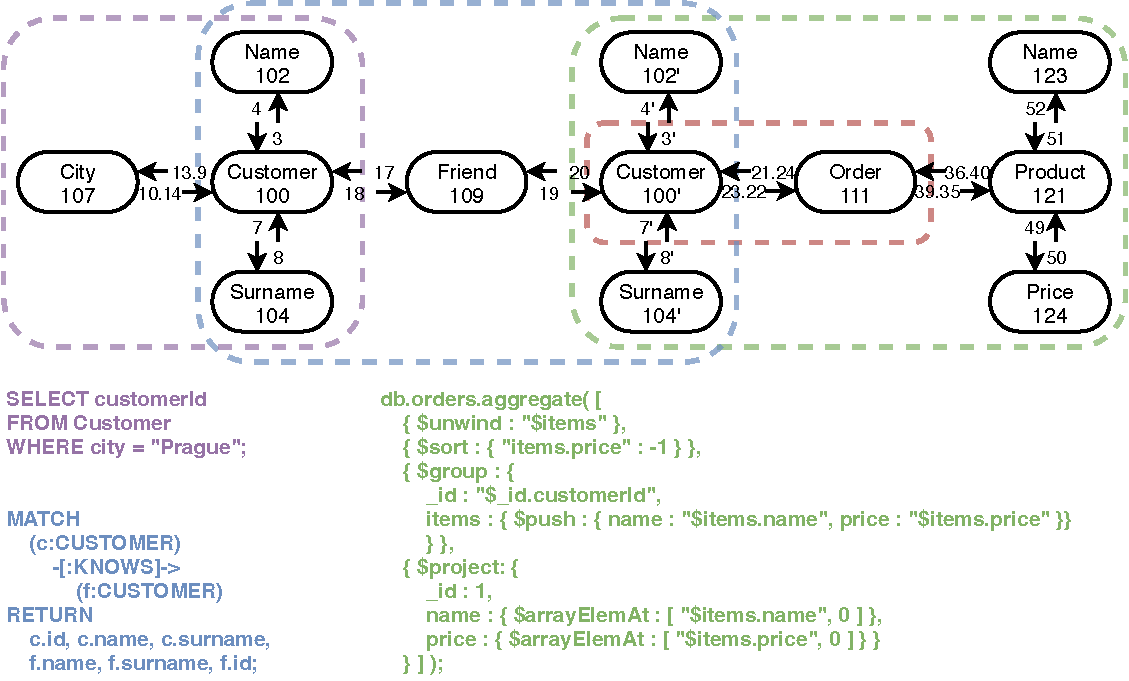
\includegraphics[width=\textwidth]{img/fig_query-decomposition.pdf} 
\caption{Query decomposition into relational (purple), graph (blue) and document (green) query parts, showing the corresponding generated native database queries for each query part~\cite{unified_representation}.}
\label{fig:querydecomposition}
\end{figure}

In~\cref{fig:querypullbacks}, we can then see how the categorical results for each query part will be joined together with pullbacks.
The first pullback joins the relational data with graph data ($P_1 = result_{REL} \bowtie_{100} result_{GRAPH}$), while the second one joins the document data with the result of the first pullback ($P_2 = P_1 \bowtie_{100'} result_{DOC}$).
As described in~\cref{algo:subsection:joinplan}, the join ordering problem is known to be hard, doubly so in multi-model scenarios, therefore it falls outside the scope of this thesis, and we leave it as part of future work on this topic.

\begin{figure}
\centering
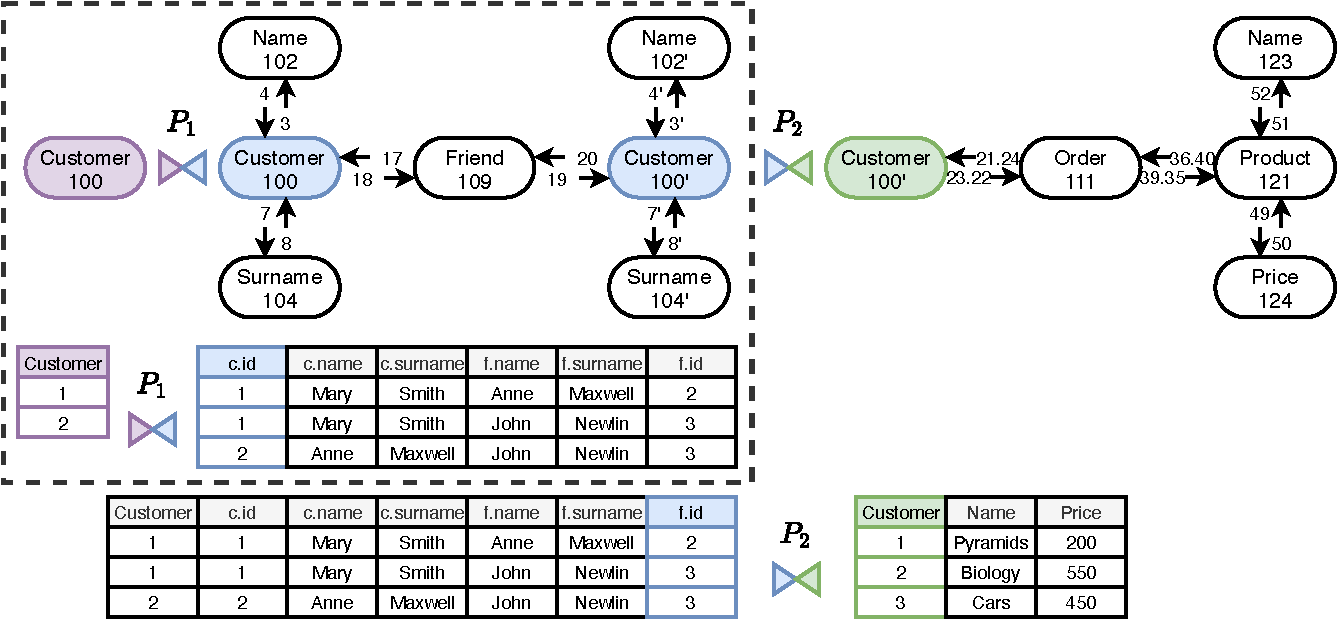
\includegraphics[width=\textwidth]{img/fig_query-join.pdf} 
\caption{Joining of query parts from~\cref{fig:querydecomposition} using pullbacks~\cite{unified_representation}.}
\label{fig:querypullbacks}
\end{figure}

\begin{figure}
\begin{code}
// PostgreSQL query
1,4,Alice
2,3,Bob
5,6,Charlie

// MongoDB query
{ customer_id: 1, price: 30 },
{ customer_id: 2, price: 25 },
{ customer_id: 3, price: 25 },
{ customer_id: 4, price: 30 },
{ customer_id: 5, price: 50 },
{ customer_id: 6, price: 10 }
\end{code}
\caption{Native query results for the queries shown in \cref{algo:fig:induced_native}.}\label{algo:fig:induced_results}
\end{figure}

For another example, we will remind the reader of the query in \cref{algo:fig:induced_query}.
Recall that in \cref{algo:fig:induced_native}, we showed the generated native queries for this MMQL query.
In \cref{algo:fig:induced_results}, we can see the results of these native queries as returned by the respective databases.
With these results, after their transformation to an instance category, we can expect to see the instance morphism $4_1$ to contain the following relations, showing relations between active domain rows of instance objects (each object active domain row is a set of tuples (signature, value)):

\begin{itemize}
    \item \texttt{(\{(6,30)\}, \{(1,1),(2,Alice)\})}
    \item \texttt{(\{(6,25)\}, \{(1,2),(2,Bob)\})}
\end{itemize}

As we can see in the first row, there is an order with a total price of $30$ which was placed by a customer with an ID of $1$ named Alice.
Let us also look at the instance morphism $4_2$:

\begin{itemize}
    \item \texttt{(\{(6,30)\}, \{(1,4),(2,Alice)\})}
    \item \texttt{(\{(6,25)\}, \{(1,3),(2,Bob)\})}
\end{itemize}

We can see that a different customer named Alice with an ID of 4 has also placed an order with a total price of $30$, and similarly, two different customers named Bob with IDs $2$ and $3$ have both placed an order with a total price of $25$.
There were also two customers named Charlie, but their orders do not have the same price, which is why they are excluded.

This approach for merging instance categories, coupled with the model-to-category transformation, leaves us with a single instance category representing the result of the MMQL \texttt{WHERE} clause.

\subsection{Projection}
\label{algo:subsection:projection}

With the instance category representing the result of the \texttt{WHERE} clause in hand, meaning we have already processed the selection part of the query, we also need to process the projection part, meaning the \texttt{SELECT} clause.
However, before we do that, there is one more thing which needs to happen -- \textit{execution of deferred statements}.
To get an overview of how this fits into the overall approach, we refer the reader to \cref{fig:queryworkflow}, whose Phase VI corresponds to the contents of this subsection.

\subsubsection{Deferred Statements}

As mentioned in~\cref{algo:subsection:transform}, there are certain MMQL statements which cross database boundaries, and therefore cannot be executed at the database level.
For example, we could have a \texttt{FILTER} statement demanding the equality of two variables whose values come from different databases.
Such statements must necessarily be processed by the MMQL query engine, and in the constraints of our approach where each query part is an executable unit independent of other query parts, this is unavoidable.
There is a possibility that for approaches which introduce dependencies between queries, a certain part of this may be optimized, for instance possibly adding a constraint to a query based on the results of another query.
However, as this is purely an optimization, we opted not to include this in our approach.

When it comes to the set of features which may possibly be a deferred statement, we have a few options, except for which all statements are \textit{not} deferred:

\begin{itemize}
    \item \textit{Triples} with repeated compound morphisms may be deferred statements in cases where the compound morphism being repeated crosses query part boundaries;
    \item \texttt{FILTER} statements may be deferred in cases where both operands of the included logic expression are variables or aggregations of variables, each of which is queried from a different database, or in cases where a required aggregation is not supported by the corresponding database; and
    \item \texttt{FILTER} and \texttt{VALUES} statements in query parts whose database wrappers define the \texttt{isNonIdFilterSupported} property to be false.
\end{itemize}

The processing of deferred statements essentially means their emulation by the query engine using the instance category corresponding to the query's \texttt{WHERE} clause.
We will not provide an explicit implementation of this algorithm, as its implementation would be lengthy and its inclusion in this thesis redundant, and all of the necessary operations are straightforward emulation of the statements.
Lastly, we will point out that the set of deferred (or deferrable) statements will vary depending on the design of the supporting algorithms for MMQL, as MMQL itself does not necessitate the deferral of any statements, opening the door to future optimizations.

\subsubsection{Projection Algorithm}

After the processing of deferred statements, we are ready to approach the main topic of this subsection, which is projection to the desired representation.
In this step, we take the instance category corresponding to the \texttt{WHERE} clause of the query, and transform it into an instance category corresponding to the \texttt{SELECT} clause, which induces its own schema category.
It is worth mentioning the construction of this schema category, as we will need the morphisms contained within to have correct cardinalities.
This can be achieved by iterating over the morphisms defined in the \texttt{SELECT} clause, and for each of them, finding all paths in the schema category induced by the \texttt{WHERE} clause between the subject and object of the triple where the morphism is defined, disregarding paths containing cycles.
We do not consider paths with cycles, as a cycle starting and ending with the same variable necessarily cannot have any effect on the cardinality of the final morphism, as it forms an identity function.
Note that there can indeed be multiple paths, for example if we consider two customers who each have a home address listed, we may have a query expressing the fact that both customers who ordered a specific item live at the same address, giving us two paths between the item ordered and the customer address.
For each morphism, we must examine all paths, selecting the minimal and maximal cardinality of the entire path, and then select the minimal value of the sets of minimal and maximal cardinalities to get the final minimal and maximal cardinality of the morphism.
This is because if multiple paths exist between the same two variables, a particular result will only be included in the instance category only if all of the paths match (unless some of those paths are optional and generated by the \texttt{OPTIONAL} clause, however we still need to consider them for the minimal and maximal calculation).
The algorithm generating the schema category induced by the \texttt{SELECT} clause can be seen in~\cref{algo:alg:projectionschema}.
We will point out the function \texttt{getPathsInSchema} used in line 10 of the aforementioned algorithm, which finds all paths in the schema category between two schema objects, provided to the function using the \texttt{src} and \texttt{dst} arguments for source and destination respectively.

\begin{algorithm}[ht]
\small
\DontPrintSemicolon
\SetKwProg{Fn}{function}{:}{}
\SetKw{return}{return}
\SetKw{break}{break}

\KwIn{$\mathbf{S}_{WHERE}$  -- schema category induced by the WHERE clause\;}
\myinput{$SELECT$  -- SELECT clause of the MMQL query\;}

$\mathbf{S}_{SELECT}$ := $\emptyset$

\ForEach{\textup{triple $subject$ $morphism$ $object$ in $SELECT$}}{
    \ForEach{\textup{$var$ in [$subject$, $object$]}}{
        $oldObj$ := $\mathbf{S}_{WHERE}$.getObjectFromVar($var$)
        
        $newObj$ := $\mathbf{S}_{SELECT}$.getObjectByKey($oldObj$.key)
        
        \If{\textup{$newObj$ is NULL}}{
            $\mathbf{S}_{SELECT}$.objects.add($oldObj$)
        }
    }

    $newMorphism$ := $\mathbf{S}_{SELECT}$.getMorphism($morphism$)

    \If{\textup{$newMorphism$ is NULL}}{
        $paths$ := getPathsInSchema($\mathbf{S}_{WHERE}$, src=$subject$, dst=$object$)

        \ForEach{\textup{$path$ in $paths$}}{
            \If{\textup{$path$ contains cycles}}{
                $paths$.remove($path$)
            }
        }

        $minCards$ := [ ]

        $maxCards$ := [ ]
        
        \ForEach{\textup{$path$ in $paths$}}{
            $minCards$.add(getMinCardinality($path$))
            
            $maxCards$.add(getMaxCardinality($path$))
        }

        $minCard$ := min($minCards$)

        $maxCard$ := min($maxCards$)

        $newMorphism$ := Morphism($morphism$, $subject$, $object$, $minCard$, $maxCard$)

        $\mathbf{S}_{SELECT}$.morphisms.add($newMorphism$)
    }
}

\caption{Projection Schema Algorithm.}
\label{algo:alg:projectionschema}
\end{algorithm}

With the schema category for the \texttt{SELECT} clause in hand, we can proceed to projecting the actual data, using the algorithm shown in~\cref{algo:alg:projectioninstance}.
This algorithm receives two inputs -- the instance category for the \texttt{WHERE} clause constructed in previous steps, and the schema category induced by the \texttt{SELECT} clause.
Its output is then data in the form of an instance category corresponding to the \texttt{SELECT} clause.
This algorithm copies over data from instance objects for the \texttt{WHERE} clause to instance objects for the \texttt{SELECT} clause (since variable projection does not modify the set of values).
It is worth explaining the notation \texttt{map($path$, $x$ $=>$ ...)} used on line 14 of \cref{algo:alg:projectioninstance}, which means the application of the lambda function in the second argument to \texttt{map} on each element of \texttt{$path$}.

\begin{algorithm}[ht]
\small
\DontPrintSemicolon
\SetKwProg{Fn}{function}{:}{}
\SetKw{return}{return}

\KwIn{$\mathbf{I}_{WHERE}$  -- instance category containing the results of the WHERE clause\;}
\myinput{$\mathbf{S}_{SELECT}$  -- schema category induced by the SELECT clause\;}

$\mathbf{I}_{SELECT}$ := $\emptyset$

\ForEach{\textup{$schemaObj$ in $\mathbf{S}_{SELECT}$.objects}}{
    $instanceObj$ := $\mathbf{I}_{WHERE}$.objects.getByKey($schemaObj$.key)

    $\mathbf{I}_{SELECT}$.objects.add($instanceObj$)
}

\ForEach{\textup{$schemaMorphism$ in $\mathbf{S}_{SELECT}$.morphisms}}{
    $subject$ := $schemaMorphism$.domain

    $object$ := $schemaMorphism$.codomain

    $paths$ := getPathsInSchema($\mathbf{S}_{WHERE}$, src=$subject$, dst=$object$)

    \ForEach{\textup{$path$ in $paths$}}{
        \If{\textup{$path$ contains cycles}}{
            $paths$.remove($path$)
        }
    }

    $instancePaths$ := [ ]

    \ForEach{\textup{$path$ in $paths$}}{
        $instancePath$ := map($path$, $x$ $=>$ getInstanceMorphism($x$, $\mathbf{I}_{WHERE}$))

        $instancePaths$.add($instancePath$)
    }

    $contractedPaths$ := map($instancePaths$, contractMorphisms)

    $instanceMorphism$ := baseInstanceMorphismIntersection($contractedPaths$)

    $instanceMorphism$.schemaMorphism := $schemaMorphism$

    $\mathbf{I}_{SELECT}$.morphisms.add($instanceMorphism$)
}

\caption{Projection Instance Algorithm.}
\label{algo:alg:projectioninstance}
\end{algorithm}

\begin{algorithm}[ht]
\small
\DontPrintSemicolon
\SetKwProg{Fn}{function}{:}{}
\SetKw{return}{return}

\KwIn{$instancePath$  -- list of base instance morphisms forming a path in the instance category induced by the WHERE clause\;}

$contractedPath$ := copy($instancePath$)

\While{\textup{len($contractedPath$) $> 1$}}{
    \tcp{If our path ends with morphisms (X) -a- (Y) -b- (Z), contract these morphisms to create a morphism (X) -a+b- (Z)}
    $b$ := $contractedPath$.popBack()

    $a$ := $contractedPath$.popBack()

    $joinedMappings$ := join($a$.mappings, $b$.mappings, $x_a$ $=>$ $x_a$.codomain, $x_b$ $=>$ $x_b$.domain)

    $contractedMappings$ := [ ]

    \ForEach{\textup{$joinedMapping$ in $joinedMappings$}}{
        $contractedMapping$ := $joinedMapping$.a.domain, $joinedMapping$.b.codomain

        $contractedMappings$.add($jcontractedMapping$)
    }

    $contractedMorphism$ := InstanceMorphism($contractedMappings$)

    $contractedPath$.add($contractedMorphism$)
}

\return{$contractedPath$.first()}

\caption{Function \texttt{contractMorphisms} from~\cref{algo:alg:projectioninstance}.}
\label{algo:alg:contractmorphisms}
\end{algorithm}

When it comes to creating the set of instance morphisms, it gets more complicated.
For morphisms from the \texttt{SELECT} clause which correspond to base morphisms from the \texttt{WHERE} clause, we can simply copy the instance morphism over to the new instance category, with a new signature corresponding to the signature specified in the \texttt{SELECT} clause.
However, it is possible for a morphism from the \texttt{SELECT} clause to correspond to a path (or set of paths) with length greater than one in the categorical representation of the \texttt{WHERE} clause.
In this case, we need to introduce the notion of \textit{morphism contractions}.
Given a compound morphism mapping a subject to an object, its contraction is a base morphism with the same mapping.
In other words, we merge the base morphisms which form the compound morphism into a single base morphism in the new instance category.
To do this, we must again get the set of paths (disregarding cycles) in the instance category induced by the \texttt{WHERE} clause, and perform morphism contraction on each path.
Finally, to produce the new instance morphism for the result instance category, we perform an intersection of all base morphisms created as a result of the path contractions, meaning the final domain-codomain map only contains a mapping of domain to codomain if all paths contain this mapping.

\subsubsection{Additional Considerations}

The perceptive reader may have noticed that the algorithm which we presented in \cref{algo:alg:projectioninstance} does not take into account the \texttt{OPTIONAL}, \texttt{UNION} and \texttt{MINUS} clauses of MMQL.
Indeed, the semantics of paths contained within these clauses are different in the context of creating result instance morphisms, however we intentionally omitted them from~\cref{algo:alg:projectioninstance} to preserve its simplicity and readability.

When it comes to paths within (or partially within) the \texttt{OPTIONAL} clause, we can disregard them if there exists at least one non-optional path, as the non-optional paths constrain the instance morphism to a set of mappings, and regardless of the existence of a particular optional mapping, the corresponding non-optional mapping always exists.
If no non-optional paths exist, then we define the instance morphism to be the union of all optional paths, after morphism contraction has been applied to them.
This is because for any given domain-codomain mapping to exist in the result instance morphism, it is enough for any given optional path to exist in the instance category corresponding to the \texttt{WHERE} clause.

Earlier, we specified that both arguments of the \texttt{UNION} clause are treated as optional.
If the entirety of a given \texttt{UNION} clause could be resolved within a single query part, we do not need to perform any extra work, as not only do we have the correct data in the instance morphisms, but the set of instance objects is also correctly filtered.
In the case that the \texttt{UNION} clause spans multiple query parts, we need to additionally filter the set of instance objects to eliminate those for whom neither \texttt{UNION} argument was matched.

As for the \texttt{MINUS} clause, the final instance morphism is the result of taking the instance morphism from the first argument of \texttt{MINUS}, while for any given domain-codomain mapping, if this mapping is also contained in the second argument of \texttt{MINUS}, it is eliminated.
Note that if the \texttt{MINUS} clause is contained entirely within a single query part, the required results have already been filtered out, meaning the filtering at this level is trivial, removing no mappings.

The last simplification made in the algorithm is the omission of constants and aggregations present in the \texttt{SELECT} clause.
While aggregations present here could be computed at the database level to increase overall efficiency, this is an optimization which would complicate the algorithms further, which is why we opted to simply explain it in this fashion.
Aggregations and constants in the \texttt{SELECT} clause would have schema objects defined just like variables, with corresponding instance objects having a constant value in the case of constants.
In the case of aggregations, their values would be computed according to their semantics as described in~\cref{mmql:subsection:grouping}, with the instance morphisms being defined accordingly.

We should also mention that the algorithms presented in this subsection are critical to query performance, as morphism contraction is an extremely expensive operation for a large dataset, entailing an inner join across all data in the instance morphism for each contraction.
The true cost of the contraction operation will be further explored in~\cref{eval}.

The final piece of the projection algorithm is taking care of the \texttt{ORDER BY}, \texttt{LIMIT} and \texttt{OFFSET} clauses of the query.
Again, while these could be handled at the database level natively, this is purely an optimization, and it would complicate the structure of our algorithms, which is why we opted to address them here.
As far as ordering is concerned, the final instance category would be divided up into maximal connected components, and these connected components ordered by the ordering criteria.
A special instance object would then be inserted into the instance category, with a morphism mapping sequence numbers from $1$ to $N$ to the connected components.
\texttt{LIMIT} and \texttt{OFFSET} are quite simple in their function, meaning we would simply restrict the result set as required.

To give a concrete example, recall the query from \cref{algo:fig:induced_query}, and the results of the generated native queries from \cref{algo:fig:induced_results}.
Given these results, the final instance category which represents the result of the MMQL query will have the following active domain rows for the \texttt{\_:shared} object:

\begin{itemize}
    \item \{(name,Alice),(price,30)\}
    \item \{(name,Bob),(price,25)\}
\end{itemize}

Again, note that each active domain row is a set of tuples (signature, value).
Normally when working with a schema category, base morphism signatures are integers which are automatically assigned, but technically a base morphism signature can be any string, which is why we allow their naming in the MMQL \texttt{SELECT} clause.

\subsection{Transforming Data}
\label{algo:subsection:transform}

As the result of the algorithm as proposed up to this point, we have an instance category corresponding to the schema category induced by the MMQL query's \texttt{SELECT} clause.
However, query results in the form of an instance category may not be practical for most use cases.
For this reason, we recognize the need for the query results to be transformed into a more suitable format, like JSON or RDF.
As MMQL is a categorical query language with categorical inputs and outputs, we believe that the transformation of data is best left out of the language itself, instead relying on supplemental query tooling to perform this job.
Despite this, we will describe our proposed approach for such a transformation, as we believe it is necessary to showcase the end-to-end validity and usability of the proposals made in this thesis.
This final part of the entire workflow corresponds to Phase VII as shown in \cref{fig:queryworkflow}.

In general, we can formalize this problem as the transformation of an instance category to a specific data model.
As we mentioned in~\cref{algo:subsection:joiningdata}, Pavel Koupil and Irena Holubov{\'a} proposed an algorithm for model-to-category transformation~\cite{unified_representation}, which we are using to transform data retrieved by native database queries into a categorical representation, and to subsequently join the data from multiple databases into a single instance category representing the \texttt{WHERE} clause of the MMQL query.
However, in the same paper, they also proposed an algorithm for a transformation in the opposite direction, meaning category-to-model (Algorithms 4 and 5 in their paper).
As it turns out, this algorithm solves exactly the problem we need to solve in order to transform the result instance category to a format like JSON or RDF.
For this reason, we propose that this algorithm be used for this transformation, and we refer the reader to the original source for more details on this algorithm.

It is worth mentioning that this transformation requires an input in the form of a mapping (recall~\cref{categorical:section:mapping}), which specifies the shape of the resulting data.
This mapping can be inferred from the shape of the MMQL \texttt{SELECT} clause in a straightforward way for some data models, for example in the graph model, we are simply transforming graph data to graph data in another representation, meaning relatively few modifications are necessary.
However, for some data models like the document model, this gets somewhat complicated.
The document model operates with tree structures, which in general do not permit lower levels of the tree to refer to upper levels.
This can pose a problem in the instance that the schema category induced by the \texttt{SELECT} clause contains back edges, forward edges or cross edges (borrowing terminology from the well-known Depth First Search algorithm), which was not an issue with graph data.

There are multiple possible solutions to the problem of transforming general directed graphs to trees~\cite{graph_tree_transform}, but we will mention two main approaches which are best suited to our use case.
The first approach is to automatically determine the schema object which will become the root of the tree, and construct a tree rooted in this schema object, replacing back, forward or cross references in the tree with object identifiers where possible, and with inlined data where not possible (for example with objects which have no identifier, such as JSON arrays).
The automatic determination of the tree root is simple in the case where the graph already forms a tree, but in the more general case, we would need to pick such a tree root based on an algorithm, for example one which would pick a tree root such that the number of edges in the tree preserved from the original graph is maximal.
The second approach would be to prompt the user to manually select the tree root when requesting a transformation which requires a root to be selected and the root cannot be determined automatically, for example when transforming to JSON when the schema category induced by the \texttt{SELECT} clause is not already a tree.
However, neither of the proposals is perfect as a transformation from a general graph to a tree necessarily carries some tradeoffs, which is why we believe that users of MMQL should try to formulate their queries to output categorical data in the shape of trees where possible.
